\documentclass[main.tex]{subfiles}

\begin{document}
\section{系统设计与实现}

%总体设计、系统组成、各层模块设计, 关键代码的解释

在本节中将介绍Chiara系统的总体设计和系统实现。在总体设计的环节将介绍系统组成和各层模块的设计,在系统实现的环节将介绍各层模块的实现原理并给出部分关键代码的解释。

\subsection{系统架构}

\begin{figure}[htbp]
    \centering
    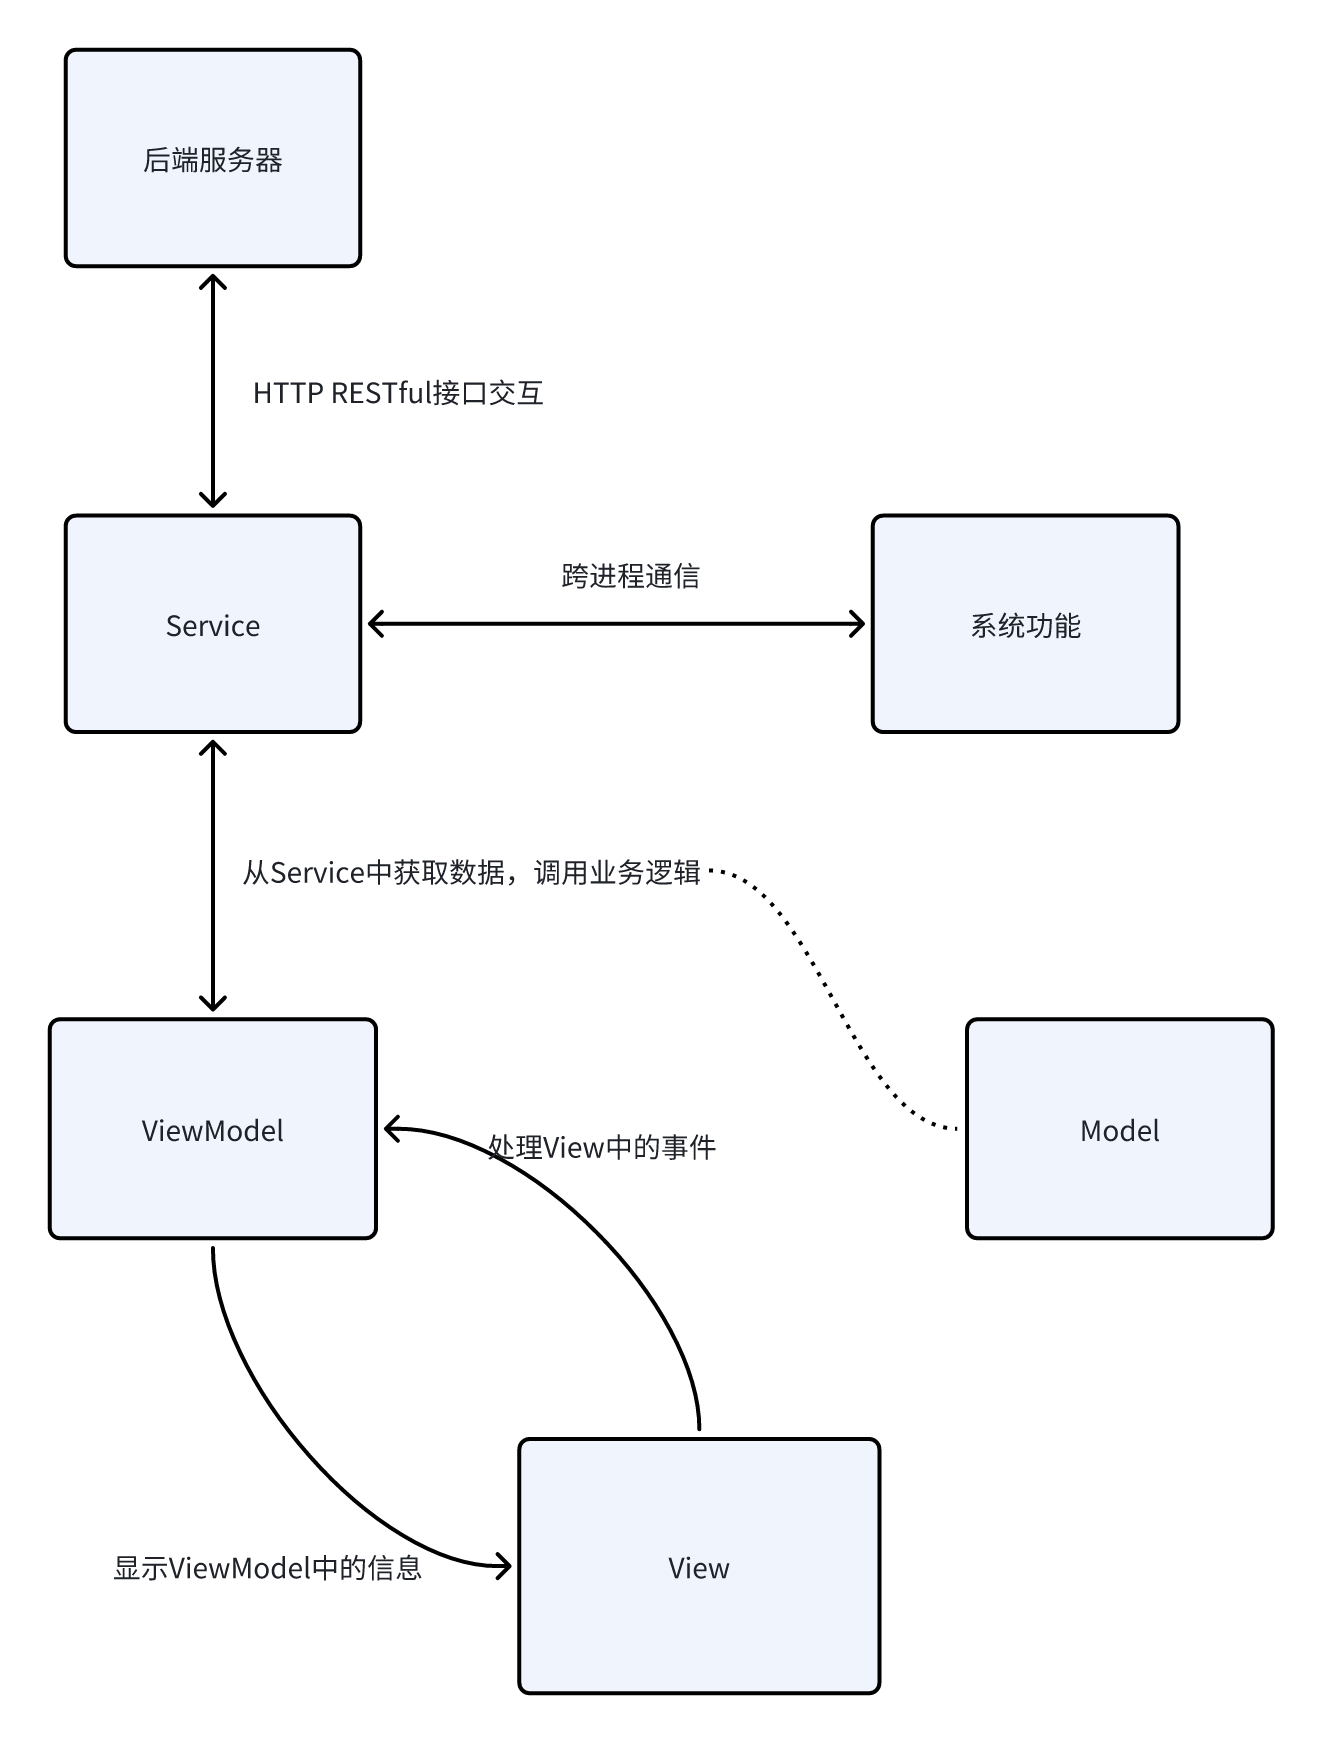
\includegraphics[width=0.75\linewidth]{assets/system-architecture.png}
    \caption{Chiara系统架构图}
    \label{fig:system-architecture}
\end{figure}

Chiara系统使用服务端/客户端的C/S架构进行开发,其中服务端软件使用ASP.NET core技术进行开发,限于作业的性质,这里不再赘述。客户端软件使用Jetpack Compose框架,按照MVVM设计模式进行开发,使用HTTP协议同后端进行通信。系统的架构如图\ref{fig:system-architecture}所示。

系统主要由如下几个部分组成:

\begin{itemize}
    \item 模型层(Model)。是系统中数据实体对象的逻辑抽象层,在视图对象和服务层交互、服务层和后端服务器交互过程中数据交互的对象。
    \item 视图层(View)。负责定义用户在屏幕上看到的结构、布局和外观。在理想情况下不包含业务逻辑;但是,在某些情况下,视图层中可能包含一下难以在视图模型层定义的交互逻辑,例如动画。
    \item 视图模型层(ViewModel)。实现视图可以数据绑定到的属性和命令,并通过更改通知事件通知视图任何状态更改。视图模型提供的属性和命令定义了要由 UI 提供的功能,但视图决定了如何显示该功能。在视图模型层调用服务层的模型时,原则是需要使用异步的调用逻辑以保持UI的响应性。
    \item 服务层(Service)。实现系统中主要的业务逻辑。在系统中典型的业务逻辑包括使用HTTP RESTful API同后端服务器进行交互;使用跨进程通信使用系统中提供的功能等等。 
\end{itemize}

\begin{figure}[htbp]
    \centering
    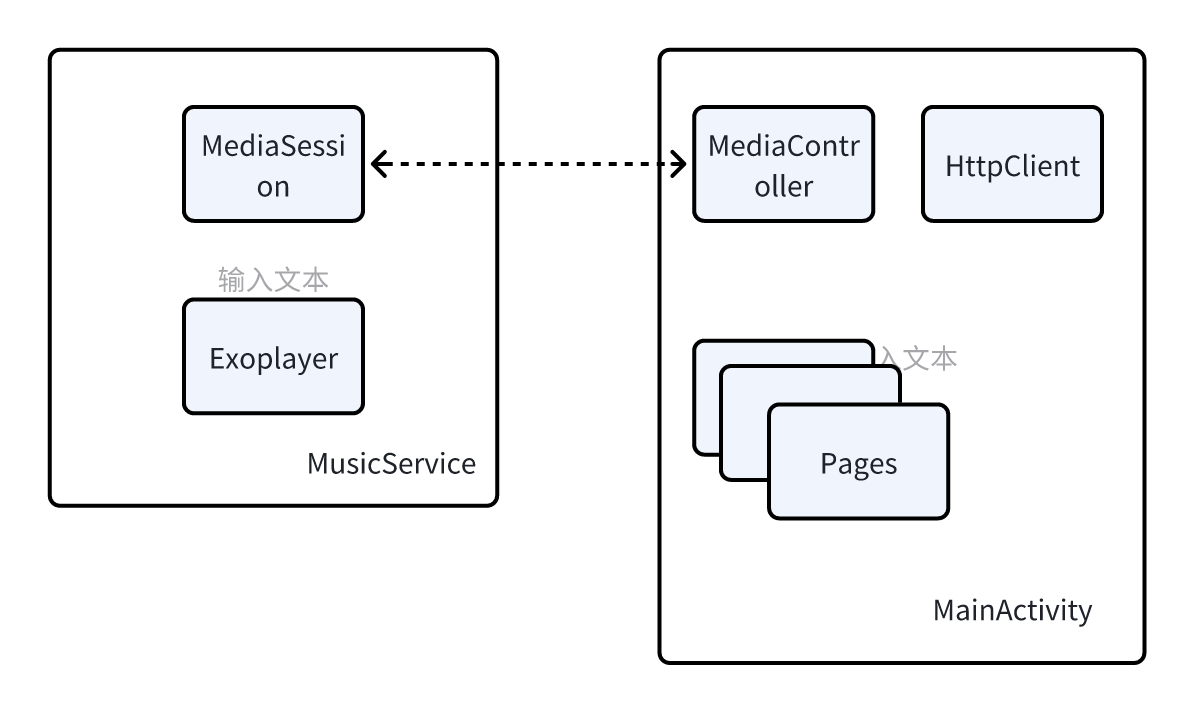
\includegraphics[width=0.8\linewidth]{assets/components.png}
    \caption{应用组件架构图}
    \label{fig:components}
\end{figure}

在Android应用系统总体还涉及到应用组件的设计,在Android系统中提供的四种应用组件中,本次系统开发使用到了其中两种,分别是Activity和Service。Activity是与用户交互的入口点,它表示具有界面的单个屏幕。Service是一种通用入口点,用于出于各种原因使应用在后台运行,它是一个在后台运行的组件,用于执行长时间运行的操作或为远程进程执行作业,Service不提供界面。系系统中的应用组件架构如图\ref{fig:components}所示。

系统中只设计了一个Activity,即Main Activity。在该Activity中设计了用户需要使用的所有界面,包括专辑查看界面,歌曲查看界面,节目查看界面,集查看界面,音乐播放界面和视频播放界面。在系统中还设计了一个Service,即MusicService。设计这个服务是考虑到音视频的编解码是一项较为繁重的工作,如果都放在MainActivity中进行运行可能会造成界面无响应并影响用户体验,同时将音乐和视频的播放放到后台服务中运行可以支持后台播放这一功能。

\subsection{分层结构设计}

\subsubsection{视图层}

视图层是系统中对于应用程序中不同页面的抽象。虽然在系统中只设计了一个Activity,但是在单个活动中仍然存在多个供展示的页面,如果将这些页面都写在同一个函数中,使用各种分支条件判断现在需要显示的内容,这将是软件工程上的灾难。因此,将页面抽象到不同的函数中是十分必要的。

在将不同的页面编写到函数之后,如何灵活地在不同的页面之间切换便是开发过程中必须要解决的问题。

在引入了导航库之后,便可以在系统的前端入口函数处定义系统中的导航信息。在定义导航信息的过程中需要给每个页面指定一个唯一的字符串作为路由,在系统的其他部分便可以利用该字符串访问对应的界面。在定义导航信息的同时,还可以定义在导航到该页面中需要携带的数据信息,例如在访问专辑页面时需要携带上一个类型为整数的专辑ID。在表\ref{tab:navigation-definion}中给出了系统中定义的页面。

\begin{table}[htbp]
    \centering
    \begin{tabular}{|c|c|c|}
        \hline
        \textbf{页面路由} & \textbf{页面函数} & \textbf{用途} \\
        \hline
         splashScreen & SplashPage & 系统的启动页面 \\
         home & Home & 系统的主页面 \\
         albumScreen & AlbumPage & 系统中显示某一专辑的页面 \\
         songScreen  & SongPage & 系统中的歌曲播放页面 \\
         playlistScreen & PlaylistPage & 系统中的播放列表 \\
         showScreen & ShowPage & 系统中显示某一节目的页面 \\
         videoScreen & VideoPage & 系统中的视频播放页面 \\
         \hline
    \end{tabular}
    \caption{导航系统的定义}
    \label{tab:navigation-definion}
\end{table}

\begin{lstlisting}[language=Kotlin]
    object Navigation {
    const val SPLASH_SCREEN = "splashScreen"
    const val HOME = "home"
    const val ALBUM_SCREEN = "albumScreen"
    const val SONG_SCREEN = "songScreen"
    const val PLAYLIST_SCREEN = "playlistScreen"
    const val SHOW_SCREEN = "showScreen"
    const val VIDEO_SCREEN = "videoScreen"
}
\end{lstlisting}

\subsubsection{视图对象层}

在MVVM架构中,负责给视图层提供数据并处理视图层发生事件的视图模型层是系统中封装主要交互逻辑的一层。在系统中,视图对象由Hilt依赖注入系统进行创建,因此可以在视图对象中访问系统的服务。同时视图对象和视图并不是一对一的关系,在系统中存在一些顶层的视图对象,例如控制播放器状态的视图对象,在\texttt{HomeBottomBar}和\texttt{SongPage}等多个组件中都会使用到。

\paragraph{MainViewModel}

系统中的顶层ViewModel,在应用初始化时便完成初始化。在该对象中,提供了当前播放器的状态\texttt{musicControllerState}和当前播放列表中的内容\texttt{playList},还提供了在系统退出时销毁播放器对象和刷新当前播放列表的功能。

\begin{lstlisting}[language=Kotlin]
@HiltViewModel
class MainViewModel @Inject constructor(
    val musicController: MusicController
) : ViewModel() {
    var musicControllerState by mutableStateOf(MusicControllerState())
        private set

    var playList: List<SongResponse> by mutableStateOf(emptyList())
        private set
\end{lstlisting}

\paragraph{HomePageViewModel} 

主页对应的ViewModel。在该对象中,提供了主页的状态\texttt{homePageState}
,还提供了切换视频和音频页面、获取远程数据等的功能。

\begin{lstlisting}[language=Kotlin]
@HiltViewModel
class AlbumPageViewModel @Inject constructor(
    apiClient: ApiClient,
    private val musicController: MusicController
) : ViewModel() {
    var albumPageState by mutableStateOf(AlbumPageState())
        private set

    private val albumApi = apiClient.createService(AlbumApi::class.java)
\end{lstlisting}

\paragraph{AlbumPageViewModel} 

专辑页面对应的ViewModel。该对象提供了专辑页面的状态\texttt{albumPageState},还提供了获得专辑信息\texttt{fetchAlbum}和选择歌曲、播放功能等一系列的功能。

\begin{lstlisting}[language=Kotlin]
@HiltViewModel
class HomePageViewModel @Inject constructor(
    private val apiClient: ApiClient
) : ViewModel() {

    var homePageState by mutableStateOf(HomePageState())
        private set
\end{lstlisting}

\paragraph{ShowPageViewModel} 

节目页面对应的ViewModel。在该对象中提供了节目页面的状态\texttt{showPageState},还提供获得节目信息的功能\texttt{fetchShowSeason}。

\begin{lstlisting}[language=Kotlin]
@HiltViewModel
class ShowPageViewModel @Inject constructor(
    apiClient: ApiClient
) : ViewModel() {
    private val showSeasonApi = apiClient.createService(SeasonApi::class.java)

    var showPageState by mutableStateOf(ShowPageState())
        private set
\end{lstlisting}

\paragraph{VideoPageViewModel} 

视频播放页对应的ViewModel。在该对象中提供了视频播放页面的状态\texttt{videoPageState}和显示提示信息栏的状态\texttt{snackBarHostState},还提供了获得视频信息并开发播放的功能。

\begin{lstlisting}[language=Kotlin]
@HiltViewModel
class VideoPageViewModel @Inject constructor(
    val musicController: MusicController,
    apiClient: ApiClient
) : ViewModel() {
    private val hlsApi = apiClient.createService(HlsApi::class.java)

    var videoPageState by mutableStateOf(VideoPageState())
        private set

    val snackBarHostState = SnackbarHostState()
\end{lstlisting}

\subsubsection{模型层}

在系统中主要存在两种对象,第一是使用OpenApiGenerator生成的,用于在服务端和客户端通信时传递信息的对象。第二是表示每个页面状态的对象。因此这里只简述第一种类,重点介绍第二种模型类。

\paragraph{专辑(Album)} 专辑是系统中对于一系列音乐的抽象。专辑中有专辑ID、专辑标题、艺术家、封面图片地址和专辑内歌曲列表等几个字段。

\paragraph{歌曲(Song)} 歌曲是系统中对于一首音乐的抽象。歌曲中有歌曲ID,歌曲标题、艺术家、封面图片地址、歌曲文件地址等几个字段。

\paragraph{节目季(ShowSeason)} 节目季是系统中对于一系列音乐的抽象。节目季中有节目ID、节目名称和节目内集列表等几个字段。

\paragraph{集(Episode)} 集是系统中对于一个视频的抽象。集中有集ID、集标题、集标号等几个字段。


\paragraph{HomePageState}

\begin{lstlisting}[language=Kotlin]
data class HomePageState(
    val loading: Boolean = false,
    val isMusicPage: Boolean = true,
    val selectedAlbum : AlbumResponse? = null,
    val errorMessage: String? = null,
    val albums: List<AlbumResponse> = emptyList(),
    val selectedSeason : ShowSeasonResponse? = null,
    val seasons: List<ShowSeasonResponse> = emptyList(),
)
\end{lstlisting}

HomePageState数据类用于表示应用首页的状态。
在该类中声明一个布尔类型的属性loading,用于指示当前页面是否正在加载数据,默认值为false。
声明一个布尔类型的属性isMusicPage,用于判断当前页面是否是音乐页面,默认值为true。
声明一个可空的AlbumResponse类型的属性selectedAlbum,用于存储用户选择的专辑信息,默认值为null。
声明一个可空的字符串类型属性errorMessage,用于存储错误消息,默认值为null。
声明一个AlbumResponse类型的列表属性albums,用于存储所有专辑信息,默认值为一个空列表。
声明一个可空的ShowSeasonResponse类型的属性selectedSeason,用于存储用户选择的季信息,默认值为null。
声明一个ShowSeasonResponse类型的列表属性seasons,用于存储所有季信息,默认值为一个空列表。

HomePageState类是为了管理系统中的首页状态,包括加载状态、是否显示音乐页面、选中的专辑、专辑列表、选中的季以及季列表等信息。

\paragraph{MusicControllerState} 

\begin{lstlisting}[language=Kotlin]
data class MusicControllerState(
    val playerState: PlayerState= PlayerState.STOPPED,
    val currentSong: SongResponse? = null,
    val currentPosition: Long = 0L,
    val totalDuration: Long = 0L,
    val repeatState : RepeatState = RepeatState.Sequence
)
\end{lstlisting}

MusicControllerState数据类,用于表示音乐播放控制器的状态。
playerState表示当前播放器的状态,默认为STOPPED。PlayerState应该是一个枚举类型,定义了播放器可能的各种状态(例如:STOPPED, PLAYING, PAUSED等)。
currentSong表示当前正在播放的歌曲信息,类型为SongResponse,这是一个可空类型,意味着在没有歌曲播放时该值可以为null。
currentPosition:表示当前播放位置的时间戳,单位是毫秒,默认值为0L。
totalDuration表示当前歌曲的总时长,同样以毫秒为单位,默认值为0L。
repeatState表示重复模式的状态,默认为Sequence。RepeatState应该也是一个枚举类型,定义了播放器的重复模式(例如:Sequence,RepeatOne,RepeatAll等)。

通过这个MusicControllerState类可以轻松地跟踪和控制音乐播放器的当前状态,包括播放状态、当前歌曲、播放位置、歌曲总时长以及重复模式等关键信息。

\paragraph{AlbumPageState}

\begin{lstlisting}[language=Kotlin]
data class AlbumPageState(
    val loading: Boolean = false,
    val selectedSong: SongResponse? = null,
    val album: AlbumResponse? = null,
    val errorMessage: String? = null
)
\end{lstlisting}

AlbumPageState数据类用于封装和管理与专辑页面相关的状态信息。
loading是一个布尔类型的字段,表示页面是否正在加载数据,默认值为false。
selectedSong是一个可空的SongResponse类型的字段,代表当前选中的歌曲信息,默认值为null。
album是一个可空的AlbumResponse类型的字段,代表当前显示的专辑信息,默认值为null。
errorMessage是一个可空的字符串类型的字段,用于存储在加载数据过程中可能出现的错误信息,默认值为null。
综上所述,AlbumPageState类用于存储专辑页面的关键状态,包括加载状态、选中的歌曲、当前专辑的信息以及任何可能发生的错误信息。

\paragraph{ShowPageState}

\begin{lstlisting}[language=Kotlin]
data class ShowPageState(
    val loading: Boolean = false,
    val showSeason: ShowSeasonResponse? = null
)
\end{lstlisting}

ShowPageState数据类包含两个字段。
loading是一个布尔型字段,表示当前页面是否处于加载状态。默认情况下,此字段被初始化为false,意味着页面加载尚未开始或已加载完成。
showSeason:是一个可空的ShowSeasonResponse类型的字段,用于存储当前显示的节目季信息。默认值为null,这可能意味着在页面加载之前或加载失败的情况下,该字段不会包含有效数据。
ShowPageState数据类用于表示与特定节目季相关的页面状态,

\paragraph{VideoPageState}

\begin{lstlisting}
data class VideoPageState(
    val loading: Boolean = false,
    val playing: Boolean = false,
)
\end{lstlisting}

VideoPageState数据类包含了两个布尔型字段。
loading表示视频页面当前是否正在加载内容,默认值为false,意味着页面加载已完成或尚未开始加载。
playing表示视频当前是否正在播放,默认值为false,意味着视频未播放或暂停状态。
VideoPageState数据类可以用来表示视频页面的状态。

\subsubsection{服务层}

系统中服务层中主要的服务为提供Exoplayer的MusicService和与之进行跨进程通信,位于MainActivity之类的MusicController以及同后端服务器进行通信的ApiClient。在上面中ApiClient是通过OpenApiGenerator生成的模板代码,封装了okhttp3的HTTP请求功能和kotlinx-serialization的JSON序列化功能,这里就不做详述。下面主要介绍MusicService和MusicController\footnote{这里虽然变量命名为Music,实际上同时负责了视频和音频的播放功能}。

\paragraph{MusicController}

MusicController使用接口的软件工程方法进行设计,分为MusicController接口和MusicControllerImpl类,后一个类实现前一个接口。这里重点介绍接口中的回调和方法。

\begin{lstlisting}[language=Kotlin]
var mediaControllerCallback: (
        (
        playerState: PlayerState,
        currentMusic: SongResponse?,
        currentPosition: Long,
        totalDuration: Long,
        repeatState: RepeatState
    ) -> Unit
)?

var mediaControllerReadyCallback: ((Player) -> Unit)?

var mediaControllerErrorCallback: ((PlaybackException) -> Unit)?
\end{lstlisting}

在MusicController中首先定义了三个回调函数,第一个回调函数负责更新当前播放器的状态,包括是否正在播放,正在播放的歌曲、正在播放的位置、 当前歌曲的总长度和播放列表的重复状态。

\begin{lstlisting}[language=Kotlin]
var player: Player?
\end{lstlisting}

在MusicController中定义了一个可以获得Player接口的字段,该类型在界面上绘制视频播放界面时会用到。

\begin{lstlisting}[language=Kotlin]
    /**
     * 添加一首曲目到播放列表中
     */
    fun addSong(song: SongResponse)

    /**
     * 添加一系列曲目到播放列表中
     */
    fun addSongRange(songs: Iterable<SongResponse>)

    /**
     * 清空播放列表
     */
    fun clearPlayList()

    /**
     * 删除播放列表中的指定曲目
     */
    fun remove(songId: Int)
\end{lstlisting}

在MusicController中定义一系列同播放列表进行交互的功能。

\begin{lstlisting}[language=Kotlin]
    /**
     * 播放播放列表中的指定曲目
     */
    fun play(songId: Int)

    /**
     * 恢复播放
     */
    fun resume()

    /**
     * 暂停
     */
    fun pause()

    /**
     * 获得当前播放歌曲的位置
     */
    fun getCurrentPosition(): Long

    /**
     * 跳转到下一首曲目
     */
    fun skipToNextSong()

    /**
     * 跳转到上一首曲目
     */
    fun skipToPreviousSong()

    /**
     * 获得当前正在播放的曲目
     */
    fun getCurrentSong(): SongResponse?

    /**
     * 跳转到指定位置
     */
    fun seekTo(position: Long)
\end{lstlisting}

MusicController定义了和播放音乐相关的一系列功能。

\begin{lstlisting}[language=Kotlin]
    fun setSequenceRepeat()

    fun setRepeatOne()

    fun setShuffleRepeat()
\end{lstlisting}


MusicController定义了设置播放列表重复逻辑的功能,包括设置顺序播放、单曲循环和随机播放。

\begin{lstlisting}[language=Kotlin]
    fun playVideo(mediaItem: MediaItem)

    fun stopVideo()
\end{lstlisting}

MusicController定义了播放视频和停止播放视频的功能。

\paragraph{MusicService}

MusicService是为实现视频和音频的后端播放,将Exoplayer对象托管给后端服务而设计了。该MusicService继承了MediaSessionService,并在类中重写了\texttt{onCreate}和\texttt{onDestroy}两个方法,在\texttt{onCreate}方法中将从依赖注入的系统中获得Exoplayer类实例,并利用该实例构建\texttt{MediaSession},这是Media3跨进程通信中的核心组件。

\begin{lstlisting}[language=Kotlin]
@AndroidEntryPoint
class MusicService : MediaSessionService() {
    private var mediaSession: MediaSession? = null

    @Inject
    lateinit var exoPlayer: ExoPlayer

    override fun onCreate() {
        super.onCreate()

        mediaSession = MediaSession.Builder(this, exoPlayer)
            .build()
    }

    override fun onGetSession(controllerInfo: MediaSession.ControllerInfo): MediaSession? {
        return mediaSession
    }

    override fun onDestroy() {
        mediaSession?.run {
            player.release()
            release()
            mediaSession = null
        }
        super.onDestroy()
    }
}
\end{lstlisting}

\subsection{关键代码段}

在本节中将重点关注系统中重点功能的核心实现细节。

\paragraph{在协程中更新播放器的状态}

\begin{lstlisting}[language=Kotlin]
init {
    musicController.mediaControllerCallback = { playerState,
                                                currentMusic,
                                                currentPosition,
                                                totalDuration,
                                                repeatState ->
        musicControllerState = musicControllerState.copy(
            playerState = playerState,
            currentSong = currentMusic,
            currentPosition = currentPosition,
            totalDuration = totalDuration,
            repeatState = repeatState
        )

        if (playerState == PlayerState.PLAYING) {
            viewModelScope.launch {
                while (true) {
                    // 每秒钟更新一次播放器的状态
                    delay(1.seconds)
                    musicControllerState = musicControllerState.copy(
                        currentPosition = musicController.getCurrentPosition()
                    )
                }
            }
        }
    }
}
\end{lstlisting}

这段Kotlin代码是在初始化MainViewModel内设置的一个媒体控制器回调,主要负责更新musicControllerState状态。
在代码中设置musicController的回调函数,当播放器状态、当前播放的音乐、播放位置、总时长或重复状态发生变化时,会调用这个匿名函数。函数参数:playerState, currentMusic, currentPosition, totalDuration, repeatState分别代表播放器状态、当前播放的音乐、当前播放位置、音乐总时长和重复模式。
在回调函数内部,首先通过\texttt{copy}方法创建一个新的MusicControllerState实例,将新的播放器状态、当前播放的音乐、播放位置、总时长和重复模式赋值给新实例的对应字段,然后将musicControllerState更新为这个新实例。这样做的目的是保持状态的不可变性,避免直接修改现有状态实例。
如果playerState为PlayerState.PLAYING(即播放器正在播放),则启动一个新的协程viewModelScope.launch,在这个协程中执行一个无限循环,每秒钟更新一次播放器的当前播放位置。具体来说,它会调用delay(1.seconds)让协程暂停一秒,然后通过musicController.getCurrentPosition()获取当前播放位置,并再次更新musicControllerState的currentPosition字段。

这段代码的核心在于如何处理播放器状态的实时更新,特别是利用Kotlin协程来实现异步和非阻塞的操作,确保UI的流畅性和响应性。同时,通过不可变数据结构(copy方法)来更新状态,有助于简化状态管理和避免潜在的并发问题。

\paragraph{依赖注入代码}

系统中的依赖注入是系统中实现服务与视图模型等各个类之间解耦的关键,下面说明系统中负责定义依赖注入的关键代码。

\begin{lstlisting}[language=Kotlin]
@Module
@InstallIn(SingletonComponent::class)
object AppModule {

    @Singleton
    @Provides
    fun provideApiClient() = ApiClient(
        baseUrl = Configuration.SERVER_ADDRESS,
        okHttpClientBuilder = OkHttpClient.Builder().readTimeout(Duration.ofSeconds(30))
    )

    @Singleton
    @Provides
    fun provideMusicController(@ApplicationContext context: Context): MusicController =
        MusicControllerImpl(context)
}
\end{lstlisting}

这段Kotlin代码定义了一个Dagger模块(AppModule),它用于提供应用程序中需要的依赖项。
\texttt{@InstallIn(SingletonComponent::class)}注解指定了当前模块提供的依赖项应该被安装到哪种类型的Dagger组件中。在这里,依赖项将被安装SingletonComponent中,意味着它们将作为单例在整个应用程序的生命周期中共享。
\texttt{@Singleton}注解表明由provideApiClient和provideMusicController函数提供的依赖项应该被创建一次并在整个应用程序中复用,即作为单例存在。
\texttt{@Provides}注解表示下面的函数是用来提供依赖项的,告诉Dagger如何实例化这些依赖项。

\texttt{provideApiClient}这个函数提供了ApiClient的实例。ApiClient的构造函数接受两个参数:baseUrl和okHttpClientBuilder。这里使用了Configuration.SERVER\_ADDRESS作为基础URL,而OkHttpClient.Builder()用于构建HTTP客户端,设置了读取超时时间为30秒。
\texttt{provideMusicController}函数提供了MusicController的实例。通过将Context作为参数传递给MusicControllerImpl的构造函数,它返回了一个MusicControllerImpl的实例,这是MusicController接口的一个实现。注意,@ApplicationContext注解表明传递的Context应该是应用程序级别的上下文,这对于访问全局资源或执行某些操作(如注册广播接收器)非常重要。

总的来说,这段代码负责配置和提供应用程序中需要的网络API客户端和音乐控制服务。

\begin{lstlisting}[language=Kotlin]
@Module
@InstallIn(ServiceComponent::class)
object ServiceModule {
    @ServiceScoped
    @Provides
    fun provideAudioAttributes() = AudioAttributes.Builder()
        .setContentType(C.AUDIO_CONTENT_TYPE_MUSIC)
        .setUsage(C.USAGE_MEDIA)
        .build()

    @ServiceScoped
    @Provides
    fun provideExoPlayer(
        @ApplicationContext context: Context,
        autoAttributes: AudioAttributes
    ) = ExoPlayer.Builder(context).build().apply {
        setAudioAttributes(autoAttributes, true)
        setHandleAudioBecomingNoisy(true)
    }
}
\end{lstlisting}

这段Kotlin代码同样是在使用Dagger框架进行依赖注入,主要为多媒体服务组件(ServiceComponent)提供必要的依赖。
\texttt{@InstallIn(ServiceComponent::class)}指定该模块的依赖项应被安装在ServiceComponent中。这意味着该模块提供的依赖将被服务组件所使用,这通常适用于多媒体应用中的后台服务或播放器服务。
\texttt{ServiceScoped}注解类似于\texttt{@Singleton},但它表示这些依赖项的生命周期将与服务组件的生命周期绑定,而不是整个应用。这在处理多媒体服务时很重要,因为服务可能在用户不交互应用时仍然运行,因此其依赖项不应在整个应用的生命周期内保持活动状态。

\texttt{provideAudioAttributes}方法提供了一个AudioAttributes的实例,它定义了音频流的属性,如内容类型和使用场景。在这里,AudioAttributes被设置为音乐类型,并且用于媒体播放。这对于控制音频流如何与其他系统音频流交互非常重要。
\texttt{provideExoPlayer}方法提供了一个ExoPlayer实例,该方法接收应用程序上下文和前面提供的AudioAttributes,然后创建并配置ExoPlayer实例。它设置了音频属性,并指示播放器在音频可能变得嘈杂时采取行动,例如当用户接电话或有其他系统声音时。

总体而言,这段代码负责为多媒体服务组件提供必要的音频属性和播放器实例。通过使用Dagger的依赖注入,它可以确保这些服务组件能够获得正确配置的依赖项,从而使得多媒体服务能够正常运行,同时保持代码的清晰和可测试性。

\paragraph{请求服务端数据}

在客户端中存在多次发起HTTP请求服务端的数据,这里选择一处获得专辑数据作为示例介绍如何完成数据的请求。

\begin{lstlisting}[language=Kotlin]
    fun fetchAlbum(albumId: Int) {
        albumPageState = albumPageState.copy(
            loading = true
        )

        viewModelScope.launch {
            val albumResponse = albumApi.apiAlbumIdGet(albumId)
            var album = albumResponse.body()

            if (albumResponse.isSuccessful && album != null) {
                album = album.copy(
                    coverImageUrl = Configuration.SERVER_ADDRESS + album.coverImageUrl,
                    songs = album.songs.map {
                        it.copy(
                            coverImageUrl = Configuration.SERVER_ADDRESS + it.coverImageUrl,
                            url = Configuration.SERVER_ADDRESS + it.url
                        )
                    }
                )

                albumPageState = albumPageState.copy(
                    loading = false,
                    album = album
                )
            } else {
                albumPageState = albumPageState.copy(
                    loading = false,
                    errorMessage = "网络错误"
                )
            }
        }
    }
\end{lstlisting}

这段Kotlin代码展示了一个函数fetchAlbum,其功能是从服务器获取特定ID的专辑信息,并更新UI状态以反映加载进度和结果。
在函数开始处,首先更新albumPageState的loading字段为true,这用于显示UI上的加载指示器。
使用viewModelScope.launch发起异步请求,这允许在后台线程上执行网络调用,而不会阻塞主线程,保证了UI的响应性。
调用albumApi.apiAlbumIdGet(albumId)执行HTTP GET请求,从服务器获取专辑详情。
使用body()方法解析响应体,尝试将其转换为Album对象。
如果请求成功(albumResponse.isSuccessful)且响应体不为空(album != null):对Album对象进行一些额外的处理,如拼接完整的图片URL和歌曲URL,这是因为服务器返回的是相对路径,需要加上服务器地址才能构成完整的URL。将处理后的Album对象存储在albumPageState中,并将loading字段设回false,表示数据加载完成。如果请求失败或响应体为空:将loading字段设为false,并设置一个错误消息errorMessage = "网络错误",这将用于向用户显示错误信息。

此函数实现了从服务器获取专辑数据的基本流程,包括启动加载状态、异步网络请求、数据处理以及UI状态更新。它还妥善处理了网络请求的错误情况,确保了用户体验的连贯性和应用程序的健壮性。使用viewModelScope和协程使得异步操作更加简洁和高效,避免了回调地狱或复杂的同步逻辑。

\paragraph{启动页面时完成初始化的工作}

在系统中进入不少页面时都需要完成初始化的工作,例如从服务段请求数据。显然,在系统中并不用在每次进入该页面时均执行一个初始化的工作,这样只会造成不必要的网络开销,降低用户使用应用的体验。下面选择进入进入专辑页面时的初始化逻辑介绍,如何只在第一次打开页面时执行一次网络请求。

\begin{lstlisting}[language=Kotlin]
composable(
    "${Navigation.ALBUM_SCREEN}/{albumId}",
    arguments = listOf(navArgument("albumId") {
        type = NavType.IntType
    })
) { backStackEntry ->
     val albumId = backStackEntry.arguments?.getInt("albumId")
    val albumPageViewModel: AlbumPageViewModel = hiltViewModel()
    val isInitialized = rememberSaveable(stateSaver = autoSaver()) {
        mutableStateOf(false)
    }
    if (!isInitialized.value) {
        LaunchedEffect(key1 = Unit) {
            albumId?.let {
                albumPageViewModel.fetchAlbum(it)
            }
            isInitialized.value = true
        }
    }
    
    AlbumPage(
        mainViewModel = mainViewModel,
        albumPageViewModel = albumPageViewModel,
        navController = navController
    )
}
\end{lstlisting}

这段代码是使用Jetpack Compose和Hilt依赖注入框架编写的一个Composable函数,用于展示专辑页面。composable函数定义了一个名为ALBUM\_SCREEN的导航目标,其路径包含一个动态参数{albumId},用于接收从上一个屏幕传来的专辑ID。然后从backStackEntry中提取albumId参数。如果参数存在,getInt("albumId")将返回对应的整数值;如果不存在,则返回null。

使用Hilt框架注入AlbumPageViewModel实例。使用rememberSaveable创建一个记忆化的状态isInitialized,初始值为false。autoSaver()自动保存和恢复状态,确保在设备配置改变(如旋转屏幕)时,状态能够正确保留。

检查isInitialized状态,如果为false,则触发数据加载过程。使用LaunchedEffect在组件初次渲染或重新创建时执行一次性的副作用,这里用于加载数据。如果albumId非空,调用fetchAlbum函数加载专辑数据。数据加载完成后,将isInitialized设为true,防止重复加载。最终调用AlbumPage Composable,传入所需的ViewModel和NavController,以显示专辑页面的内容。

此代码片段展示了如何在Jetpack Compose中定义和处理导航目标,使用Hilt注入ViewModel,以及如何在页面加载时延迟加载数据。这种模式确保了数据加载的效率和UI的响应性,同时利用Hilt和Compose的特性简化了代码结构。

\paragraph{播放动画的实现}

\begin{figure}[htbp]
    \centering
    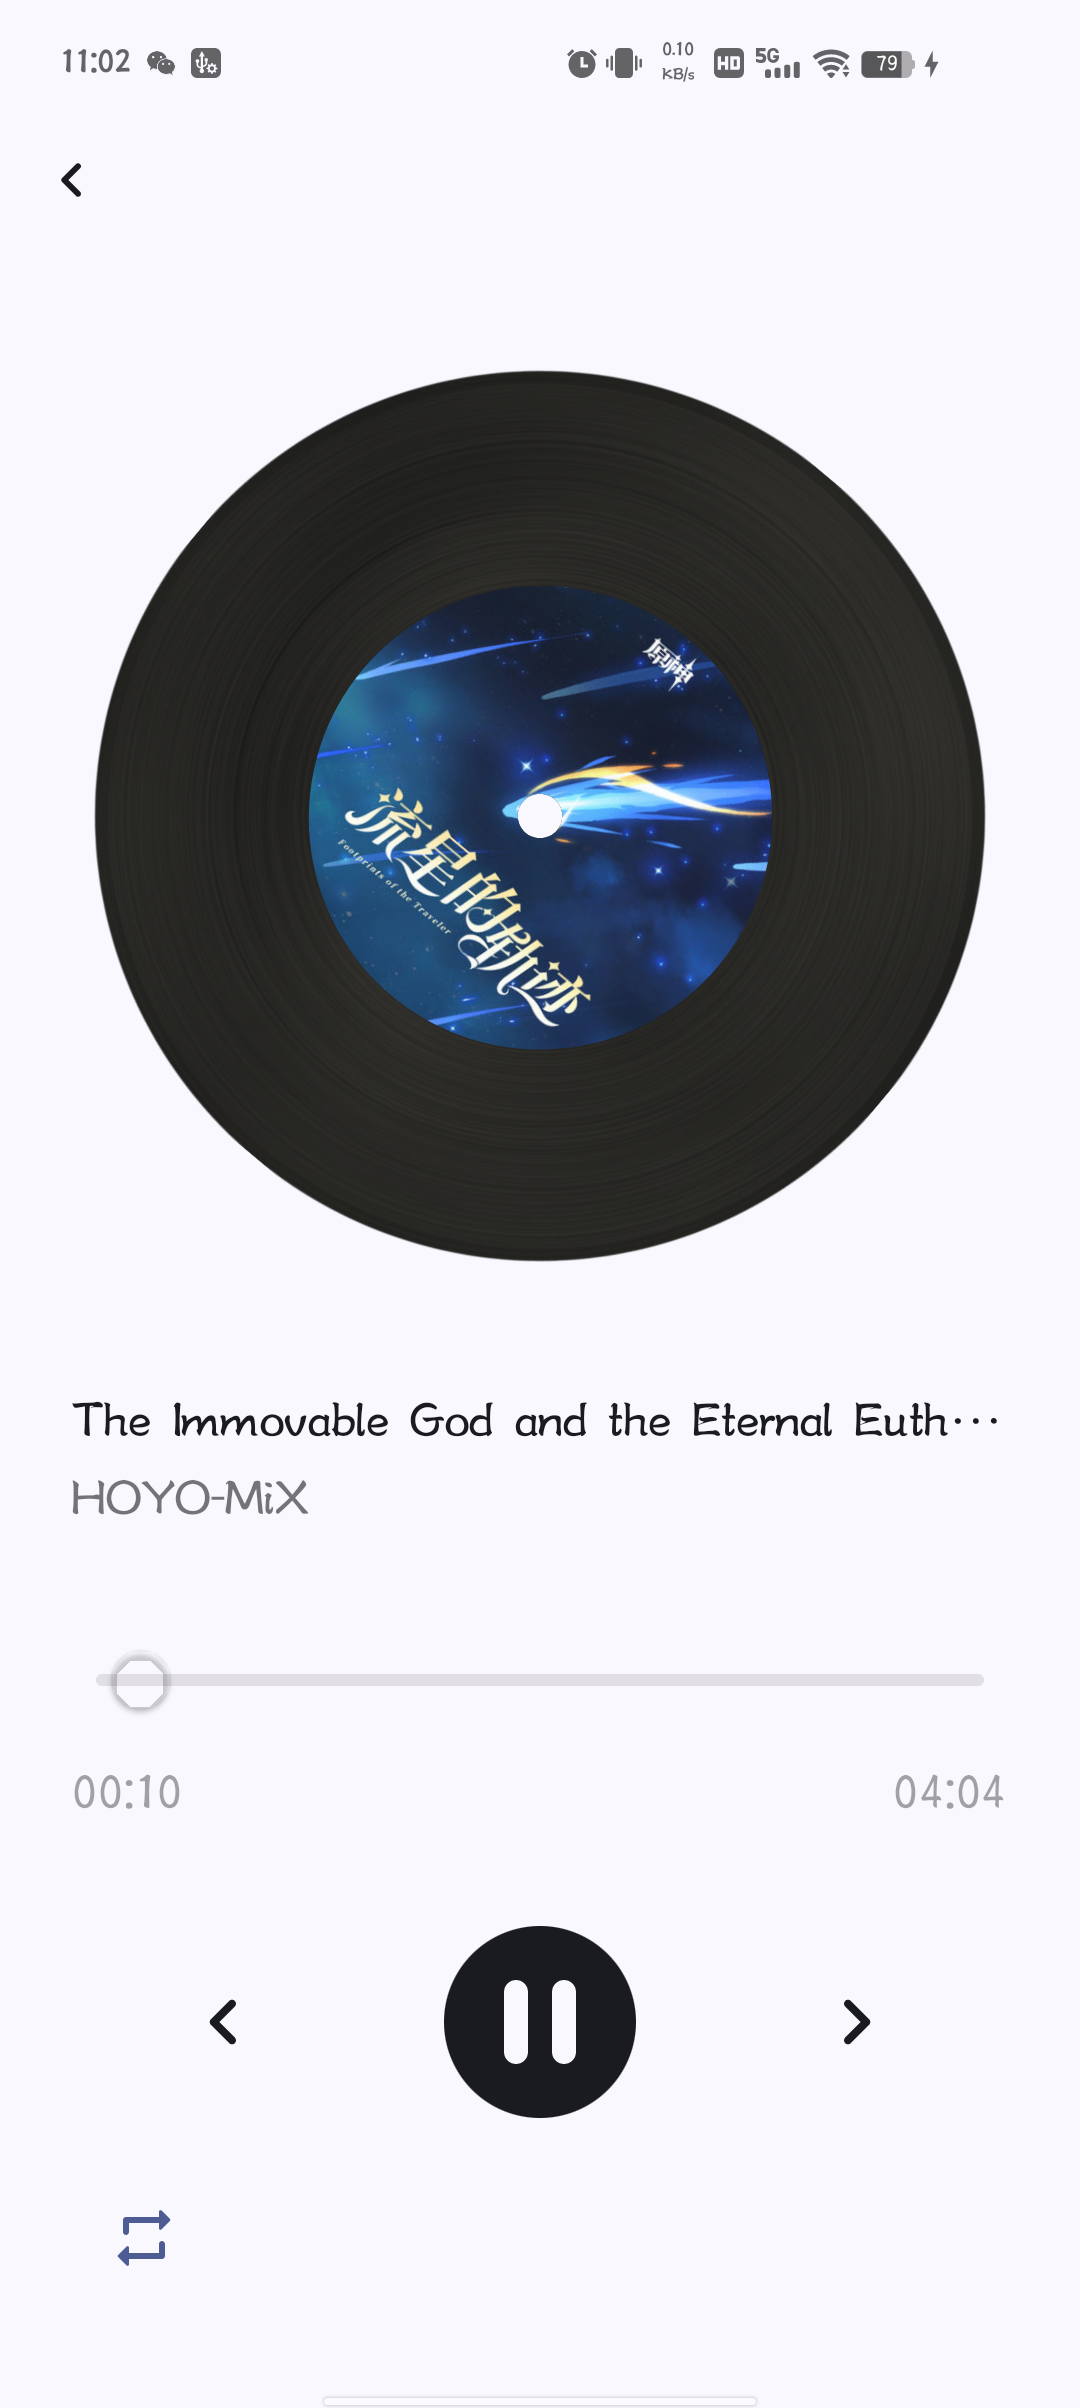
\includegraphics[width=0.4\linewidth]{assets/song-playing.png}
    \caption{播放歌曲的动画}
    \label{fig:song-playing}
\end{figure}

如图\ref{fig:song-playing}所示,在系统中设计了一个播放歌曲时的动画,下面的代码段解释了如何在程序中实现该动画效果。

\begin{lstlisting}[language=Kotlin]
@Composable
fun AnimatedVinyl(
    modifier: Modifier = Modifier,
    isSongPlaying: Boolean = false,
    painter: Painter
) {
    var currentRotation by remember {
        mutableFloatStateOf(0f)
    }

    val rotation = remember {
        Animatable(currentRotation)
    }

    LaunchedEffect(isSongPlaying) {
        if (isSongPlaying) {
            rotation.animateTo(
                targetValue = currentRotation + 360f, animationSpec = infiniteRepeatable(
                    animation = tween(3000, easing = LinearEasing),
                    repeatMode = RepeatMode.Restart
                )
            ) {
                currentRotation = value
            }
        } else {
            if (currentRotation > 0f) {
                rotation.animateTo(
                    targetValue = currentRotation + 50f, animationSpec = tween(
                        1250, easing = LinearEasing
                    )
                ) {
                    currentRotation = value
                }
            }
        }
    }

    Vinyl(modifier = modifier, painter = painter, rotationDegrees = rotation.value)
}
\end{lstlisting}

这段代码定义了一个名为AnimatedVinyl的Jetpack Compose Composable函数,用于展示一个动画化的黑胶唱片界面,其行为和外观随歌曲播放状态变化。函数的参数有: modifier:允许外部传入一个Modifier,用于自定义布局和样式。isSongPlaying:一个布尔值,指示歌曲是否正在播放,影响动画行为。painter:一个Painter对象,用于绘制黑胶唱片的图像。

在代码中使用remember创建一个记忆化的浮点型状态currentRotation,用于存储当前的旋转角度。创建一个Animatable对象,用于动画的平滑过渡,初始值为currentRotation。当isSongPlaying的值发生变化时,触发动画逻辑的执行。如果歌曲开始播放,启动无限循环的动画,使唱片连续旋转360度。其中动画的规格为动画持续时间3秒,采用线性缓动,无限循环重启。
如果歌曲停止播放,动画停止,并将唱片旋转至稍微超过起始位置的角度,以模拟惯性效果。
最后调用Vinyl Composable,传入必要的参数,包括modifier、painter和当前的旋转角度,以绘制旋转的黑胶唱片图像。

AnimatedVinyl通过结合remember、Animatable和LaunchedEffect,实现了基于歌曲播放状态的动态黑胶唱片动画。当歌曲播放时,唱片连续旋转;当歌曲暂停或停止时,动画平滑减速并停止。这种动画不仅增强了用户体验,还有效地反映了歌曲播放的状态,使得UI更加生动和直观。

\subsection{系统界面设计}

在本节中将主要介绍系统中各个页面的设计逻辑和交互方式。

图\ref{fig:main-page}展示了系统中的主页面。主页面按照典型的移动应用布局进行设计,分成顶部栏、中间内容和底部栏三个部分。

\begin{figure}[htbp]
    \centering
    \begin{subfigure}{0.45\linewidth}
        \centering
        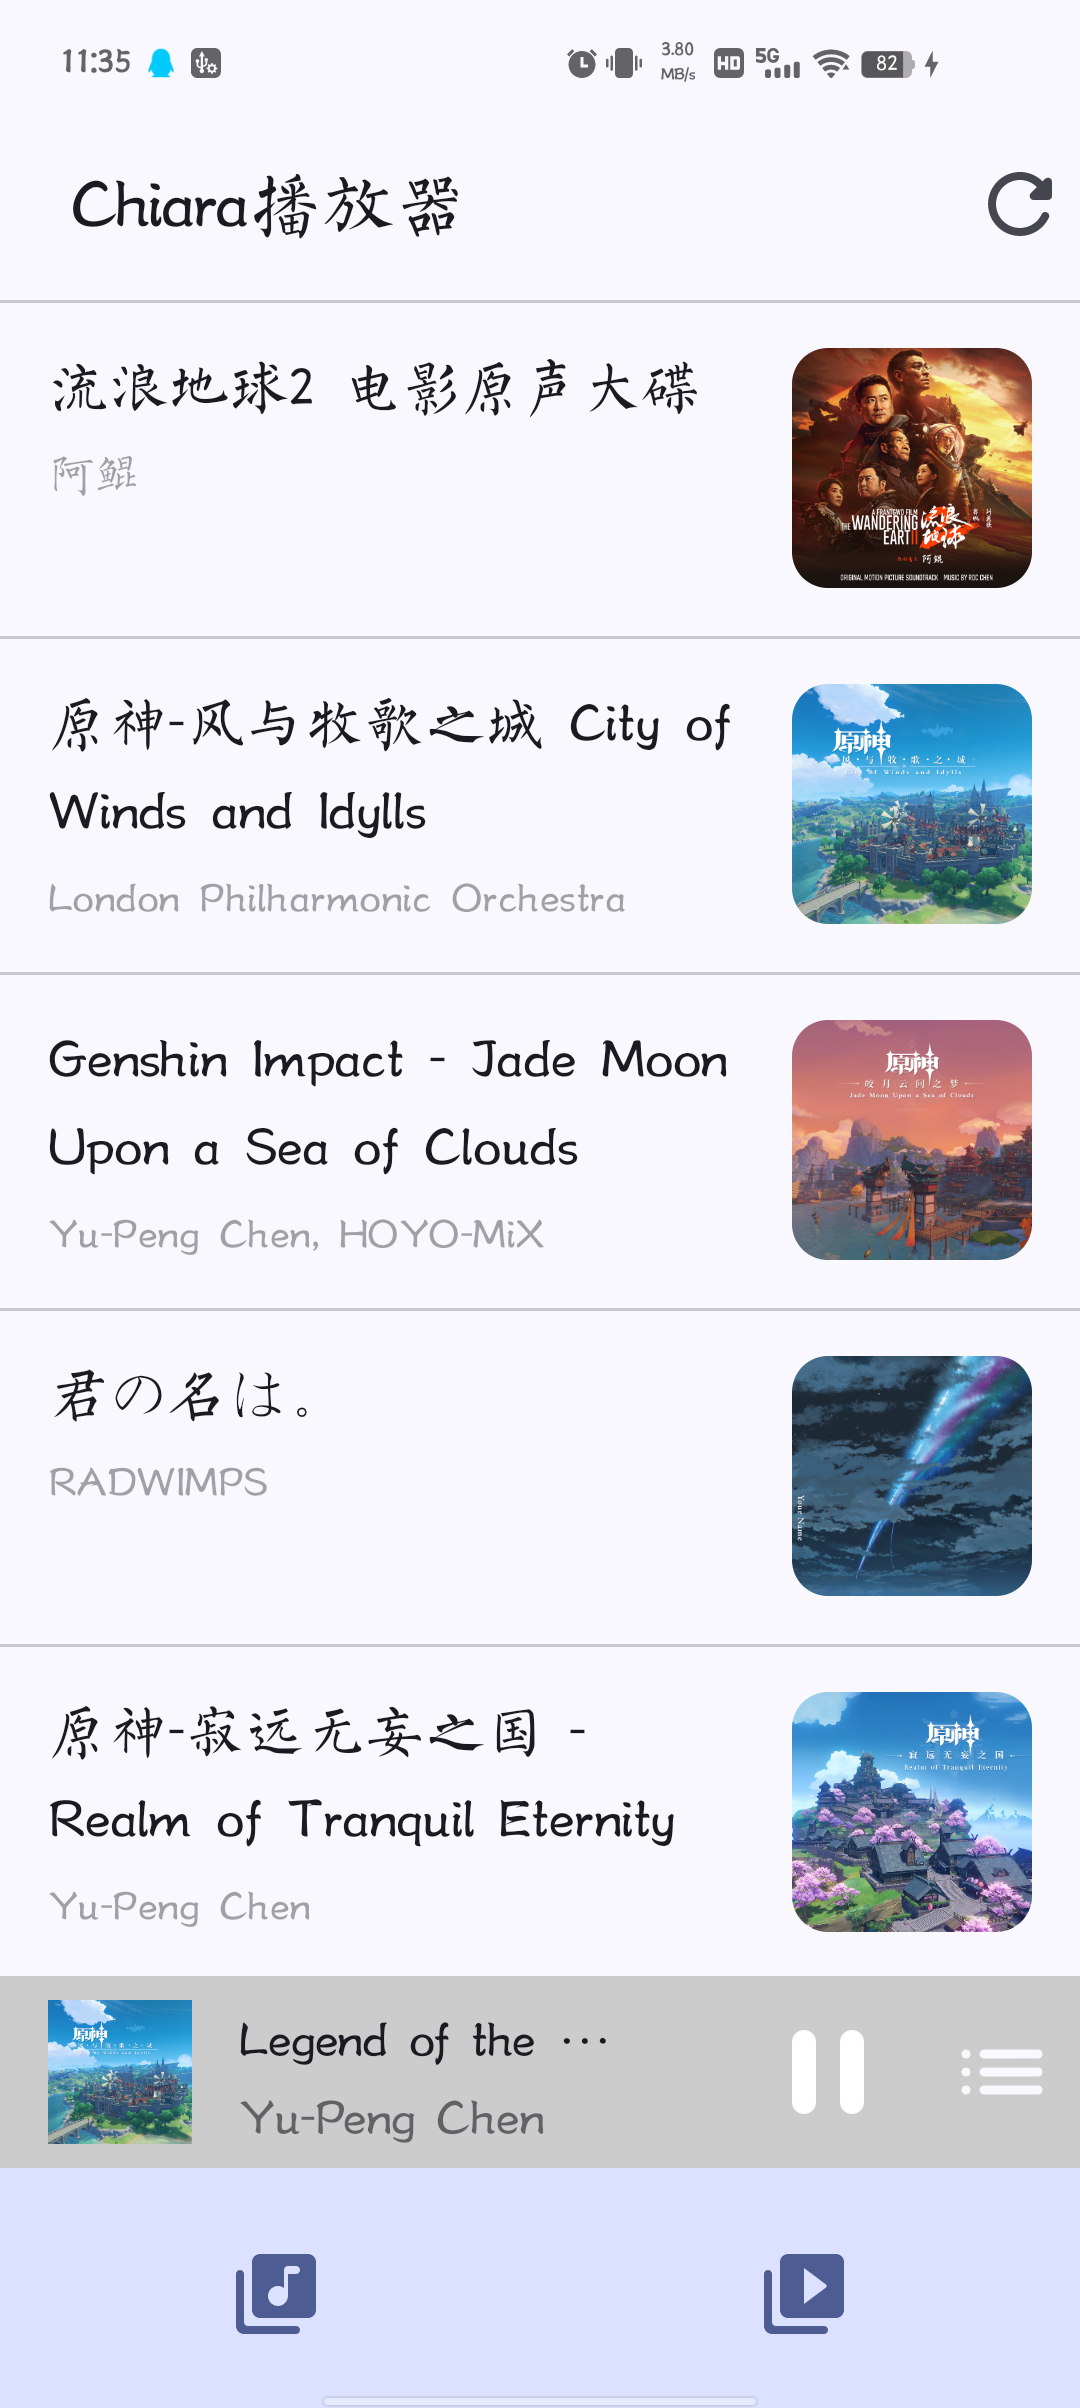
\includegraphics[width=0.9\linewidth]{assets/main-music-page.png}
        \caption{展示音乐列表时}
    \end{subfigure}
    \begin{subfigure}{0.45\linewidth}
        \centering
        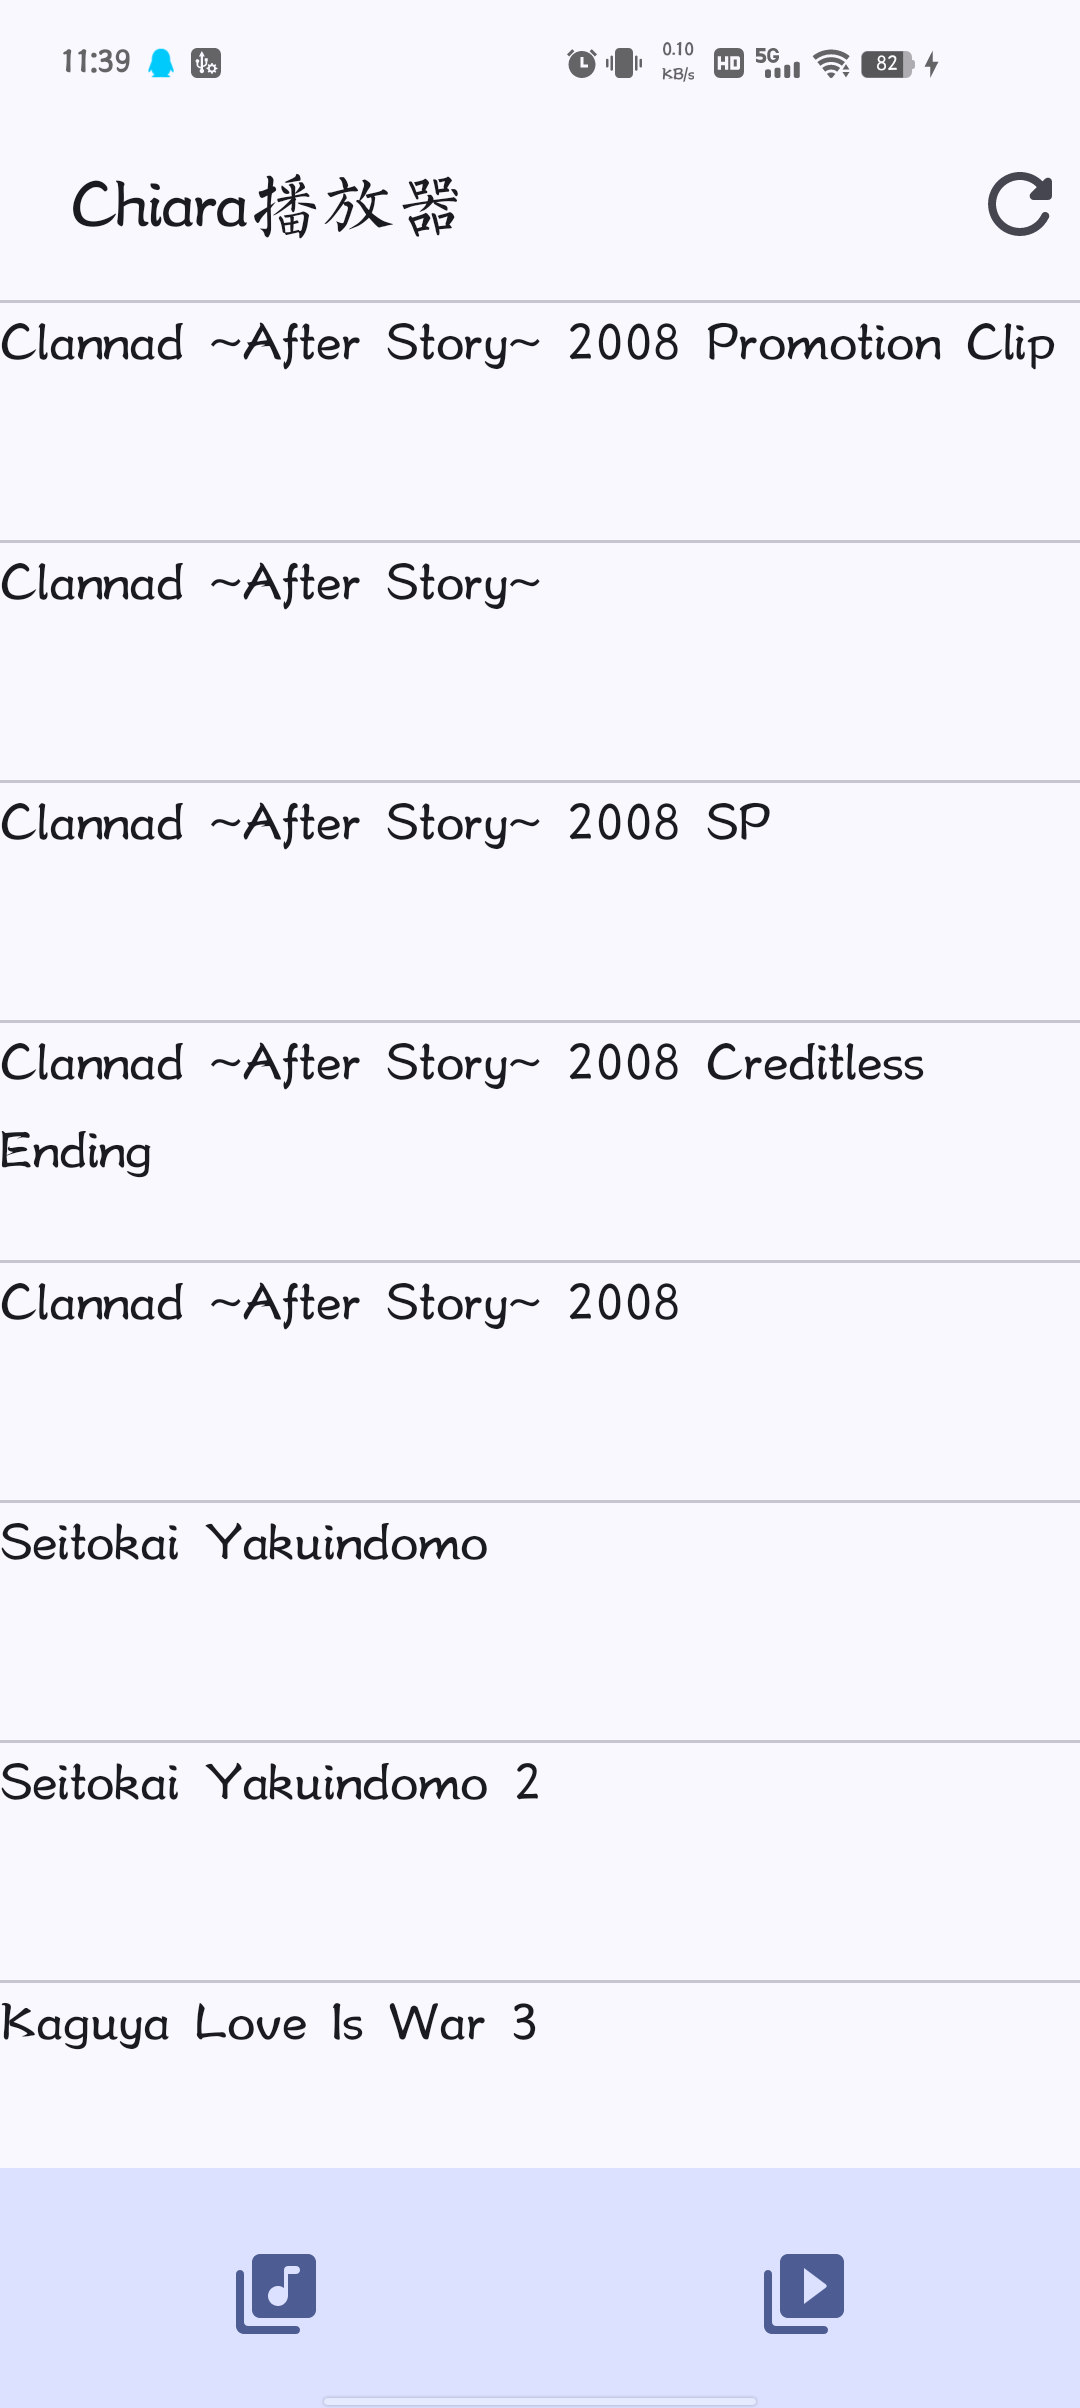
\includegraphics[width=0.9\linewidth]{assets/main-video-page.png}
        \caption{展示视频列表时}
    \end{subfigure}
    \caption{主页}
    \label{fig:main-page}
\end{figure}

顶部栏展示了当前应用的名称和一个供用户手动刷新服务端数据的按钮,在按下按钮之后系统会再次从服务端中获取音乐和视频的数据。中间部分是一个列表,展示了当前系统中所有的音乐专辑或者视频列表。如果当前为显示专辑,则在每一栏中,展示了每个专辑的标题,艺术家和专辑的封面,其中针对没有扫描或者识别到封面的专业,系统提供了一个默认的封面图片;如果当前是视频列表,当前则会展示每个节目的名称。页面的底部栏由两个部分组成,第一个部分是展示当前音乐播放转状态的播放栏,提供了快捷播放和暂停的切换按钮和进入播放列表页面的按钮。第二部分是切换当前显示系统中的专辑列表或者是视频列表。在进入视频列表页面之后,播放栏会被自动隐藏。

在点击任意专辑之后,会进入专辑内容的展示页面,如图\ref{fig:album-page}所示。

\begin{figure}[htbp]
    \centering
    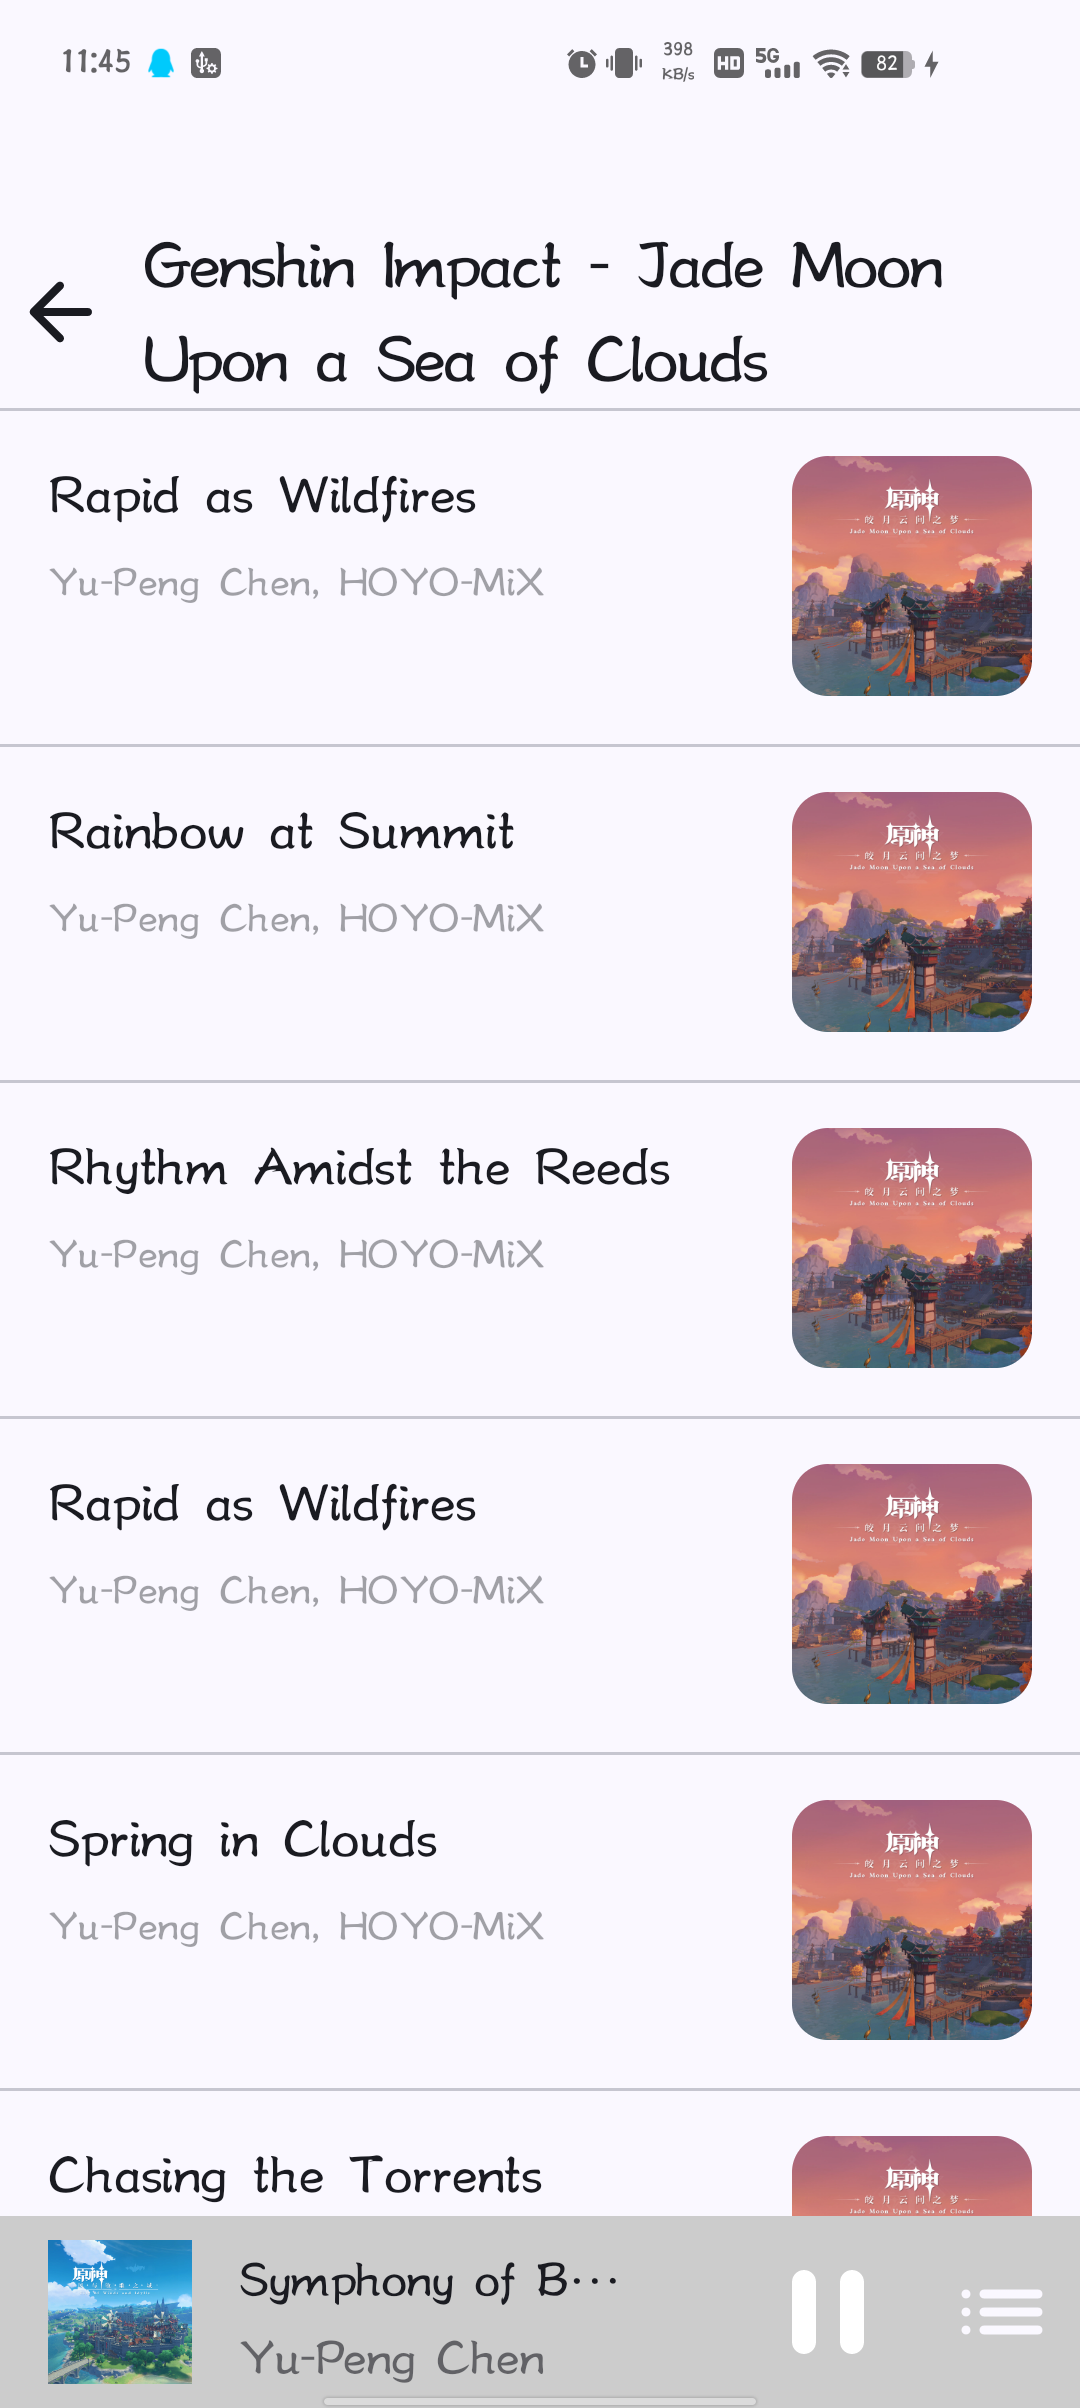
\includegraphics[width=0.4\linewidth]{assets/album-page.png}
    \caption{专辑页面}
    \label{fig:album-page}
\end{figure}

专辑页面在页面框架上保持和主页的一致性,仍然由三个部分组成。标题栏负责显示当前专辑的名称和一个返回上一页的按钮。内容部分是一个展示当前专辑内所有音乐的列表,列表中每一栏展示的信息为每首歌曲的名称、该歌曲的歌手和一张该歌曲的图片。底部栏则只有一个展示当前播放状态的播放栏。

在页面上不论是点击歌曲还是点击播放状态栏都会进入到歌曲播放的页面。歌曲播放的页面如图所示。

\begin{figure}[htbp]
    \centering
    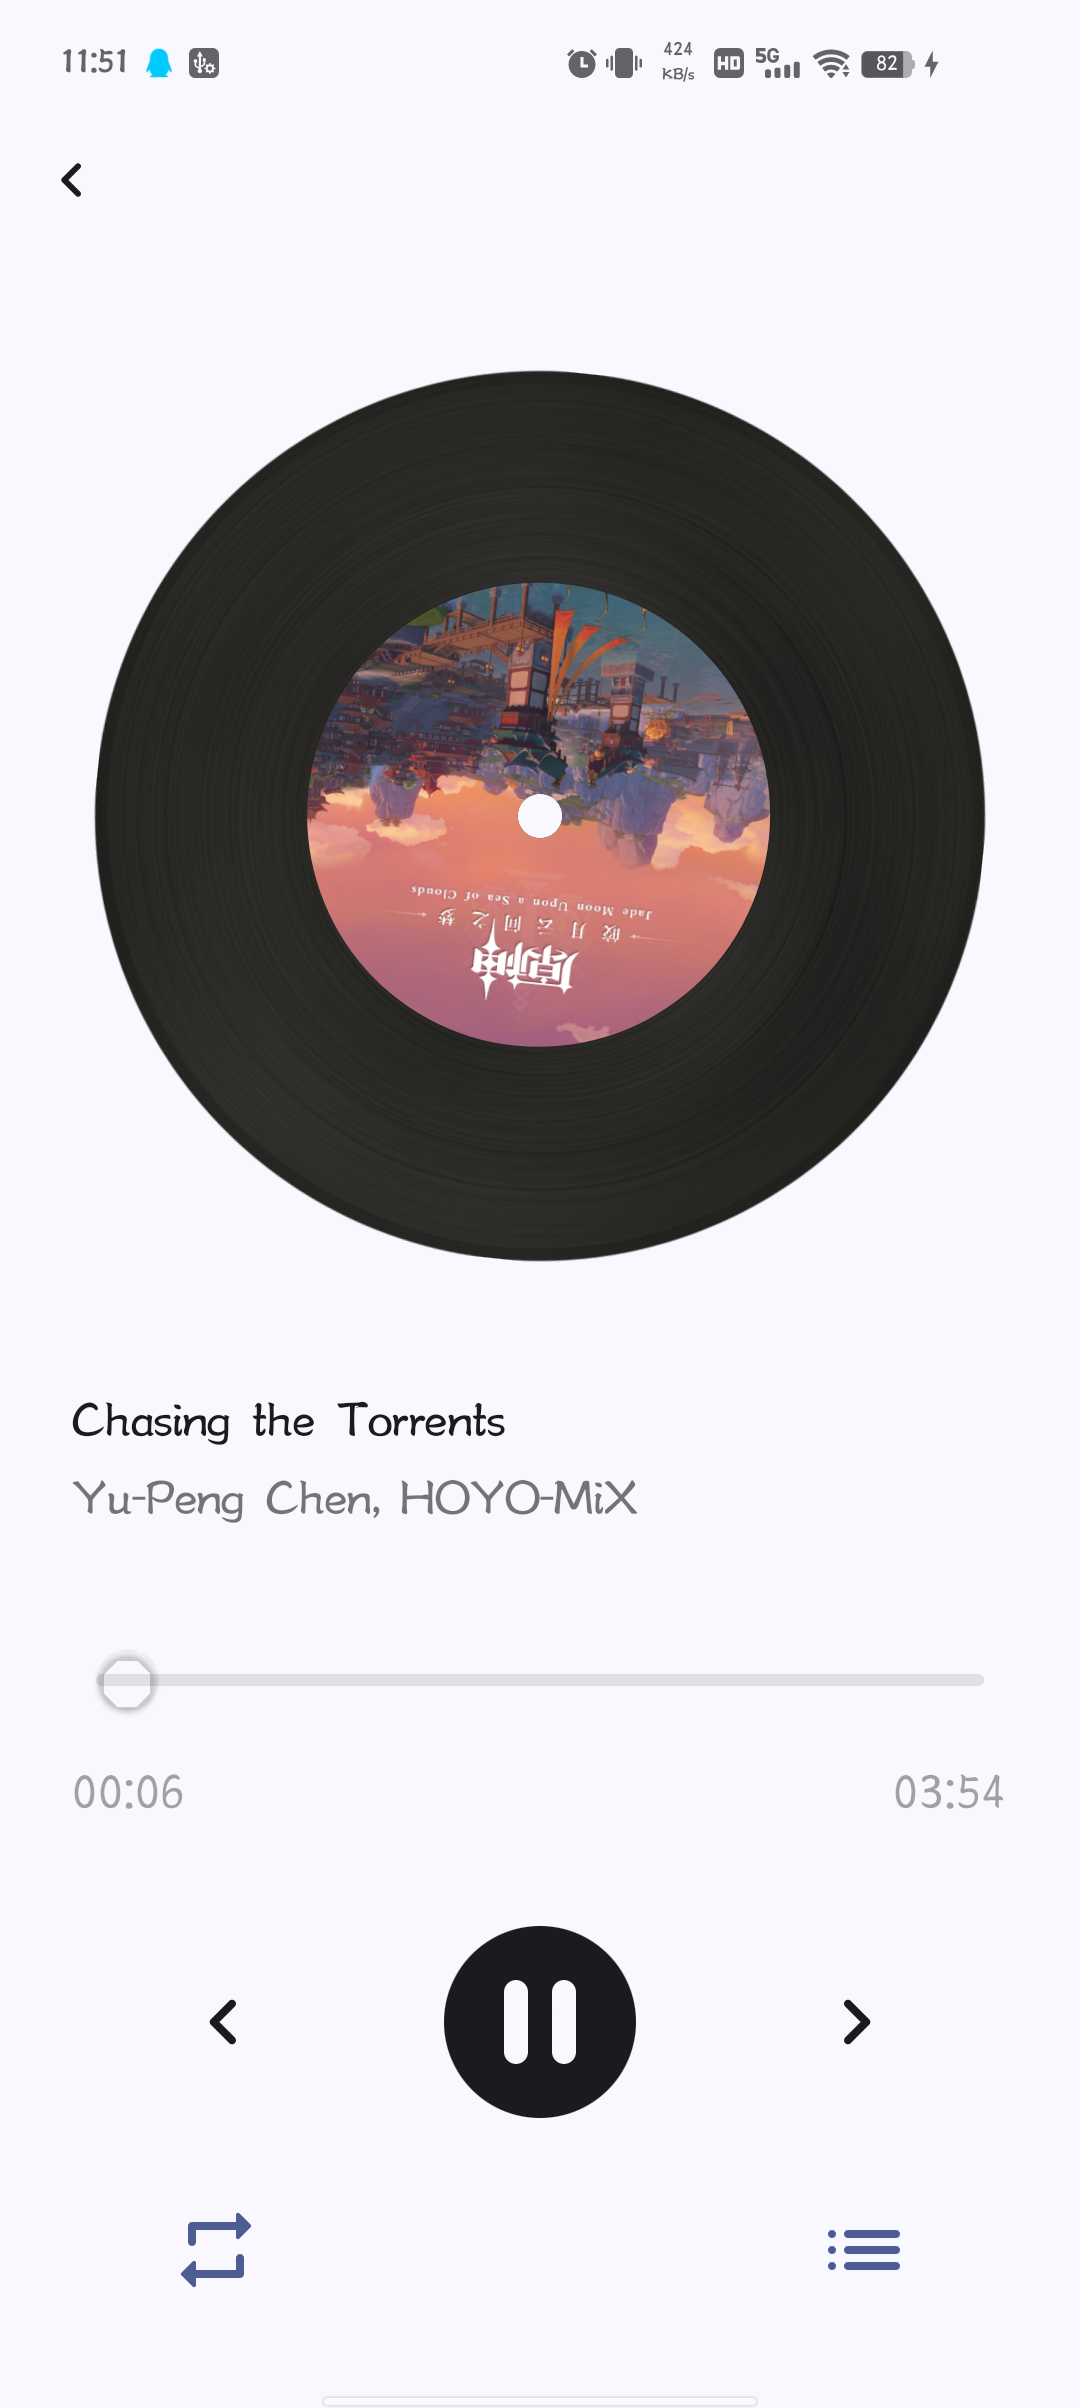
\includegraphics[width=0.4\linewidth]{assets/song-page.png}
    \caption{歌曲播放界面}
    \label{fig:song-page}
\end{figure}

歌曲播放界面专注于展示同歌曲播放相关的信息。左上角提供了一个返回上一界面的按钮,可以返回到之前的界面。中间是一张模拟黑胶唱片的动画,会在音乐播放时转动,在暂停音乐播放时停止。接下来的两行字展示了当前正在播放的音乐名称和歌手。最后便是两排控制音乐播放的功能按钮,第一行从左到右是上一首歌曲,播放暂停切换按钮和下一首歌曲按钮,第二行从左到右是切换播放模式按钮和进入播放页面按钮。其中按下切换播放模式按钮会在播放器的三种播放模式之间循环,依次为顺序播放模式、单曲循环播放模式和随机播放模式,随着播放模式的变化,界面上显示的按钮图标也会发生对应的变化。

点击在歌曲播放页面的播放列表按钮和播放状态栏上的播放列表按钮都会进入到的播放列表页面中。播放列表页面如图\ref{fig:playlist-page}所示。

\begin{figure}[htbp]
    \centering
    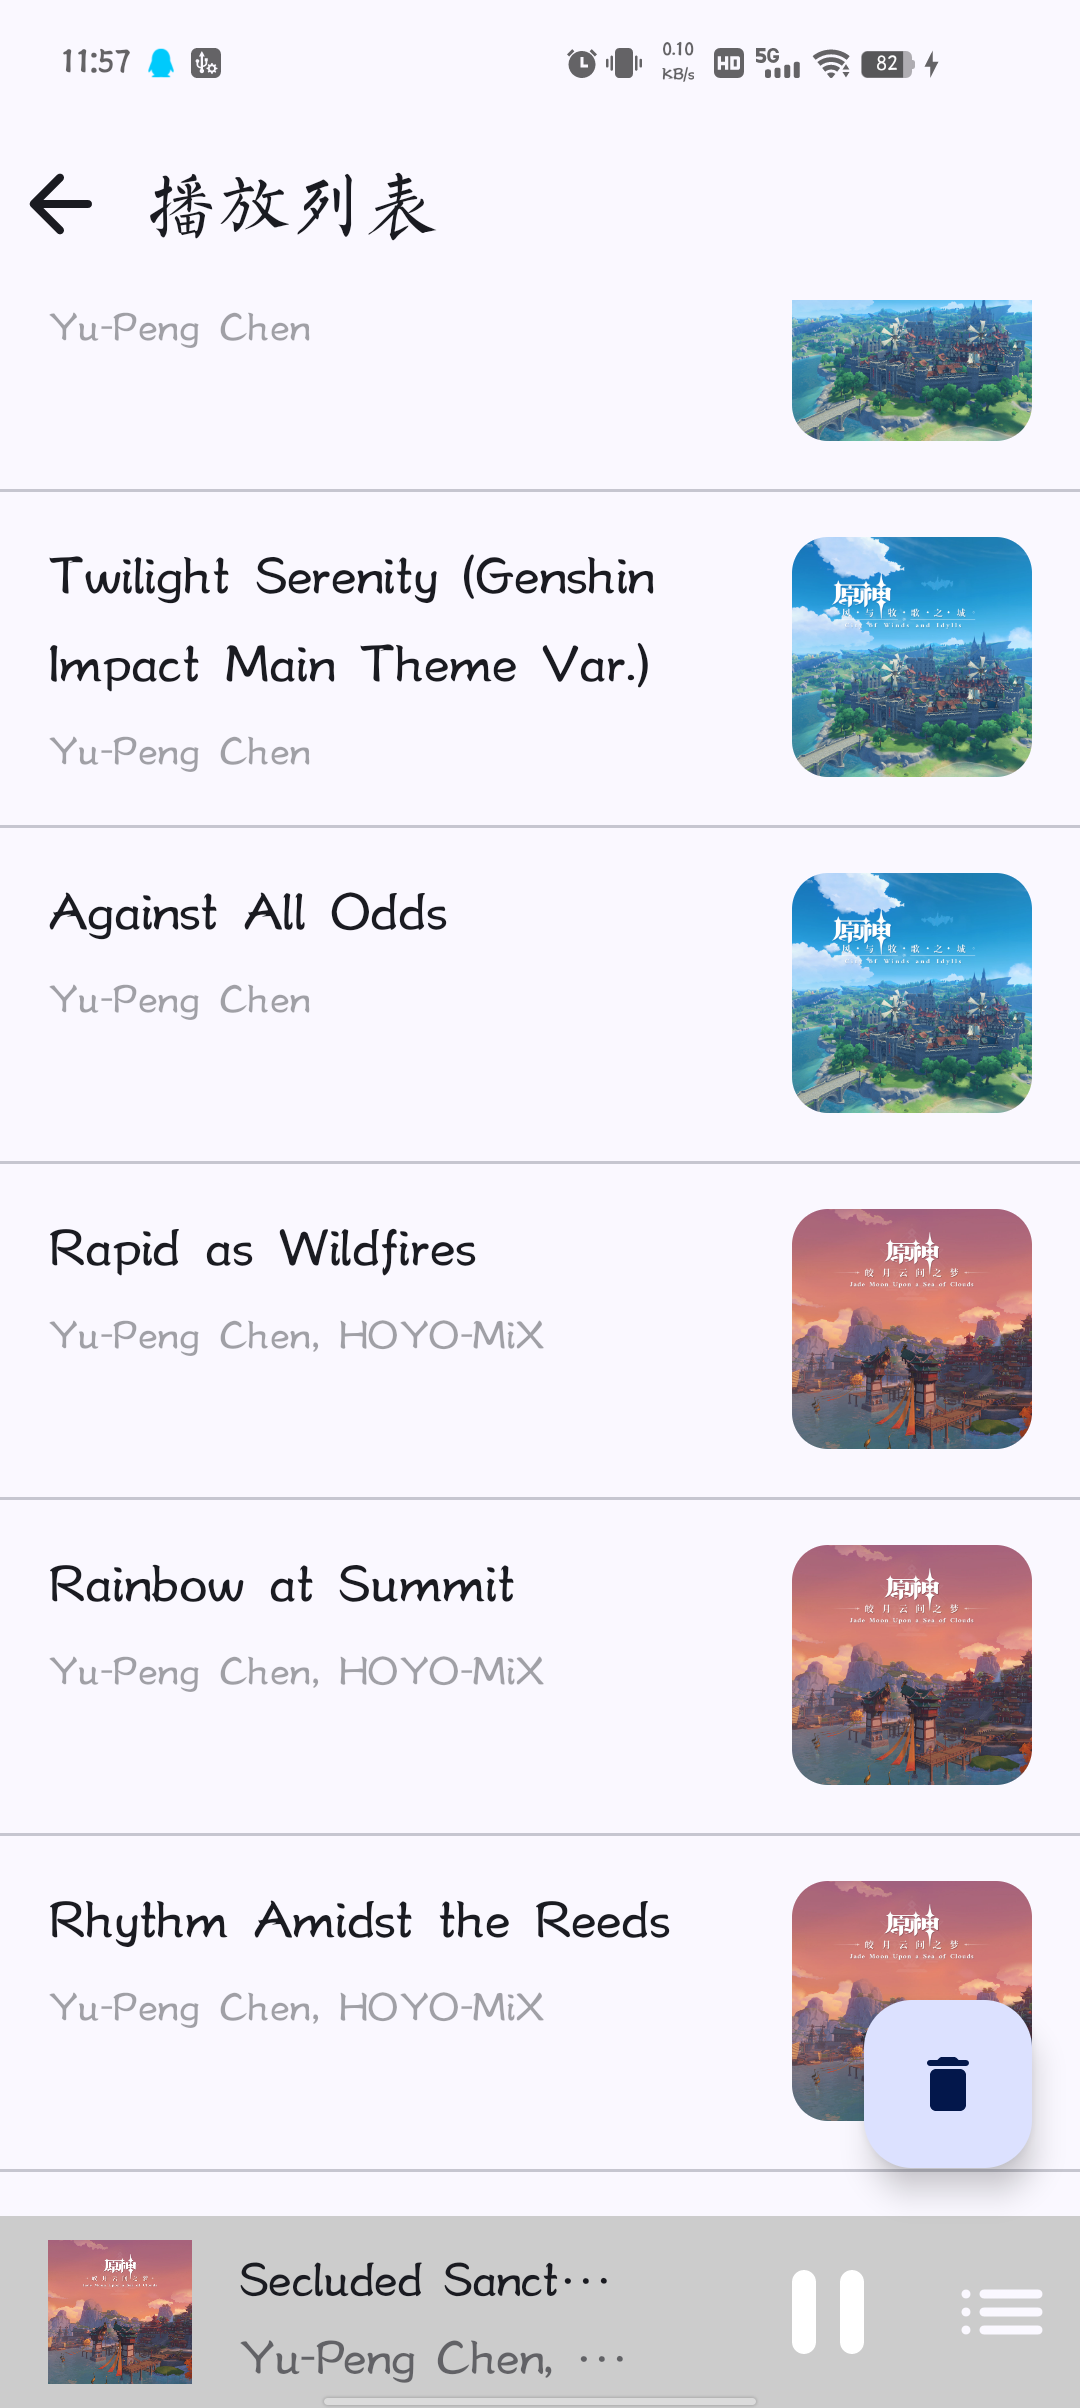
\includegraphics[width=0.4\linewidth]{assets/playlist-page.png}
    \caption{播放列表页面}
    \label{fig:playlist-page}
\end{figure}

播放列表页面仍然保持和整个系统类似的布局风格,仍然分成上中下三个部分。标题栏显示了当前页面的标题和一个返回上一页面的按钮,中间的内容列表展示了当前播放列表中的所有歌曲,其中会高亮显示当前正在播放的歌曲,每首歌曲展示的信息和专辑页面相同。最下面的状态栏为当前正在播放歌曲的状态栏。在页面的右下角提供了一个清空当前播放列表的按钮,在按下该按钮之后就会停止当前正在播放的音乐并清空当前播放器中的播放列表。

在主页中展示视频列表时点击视频列表中的任意一个节目,将会进入到节目展示页面。节目展示页面如图\ref{fig:show-page}所示。

\begin{figure}[htbp]
    \centering
    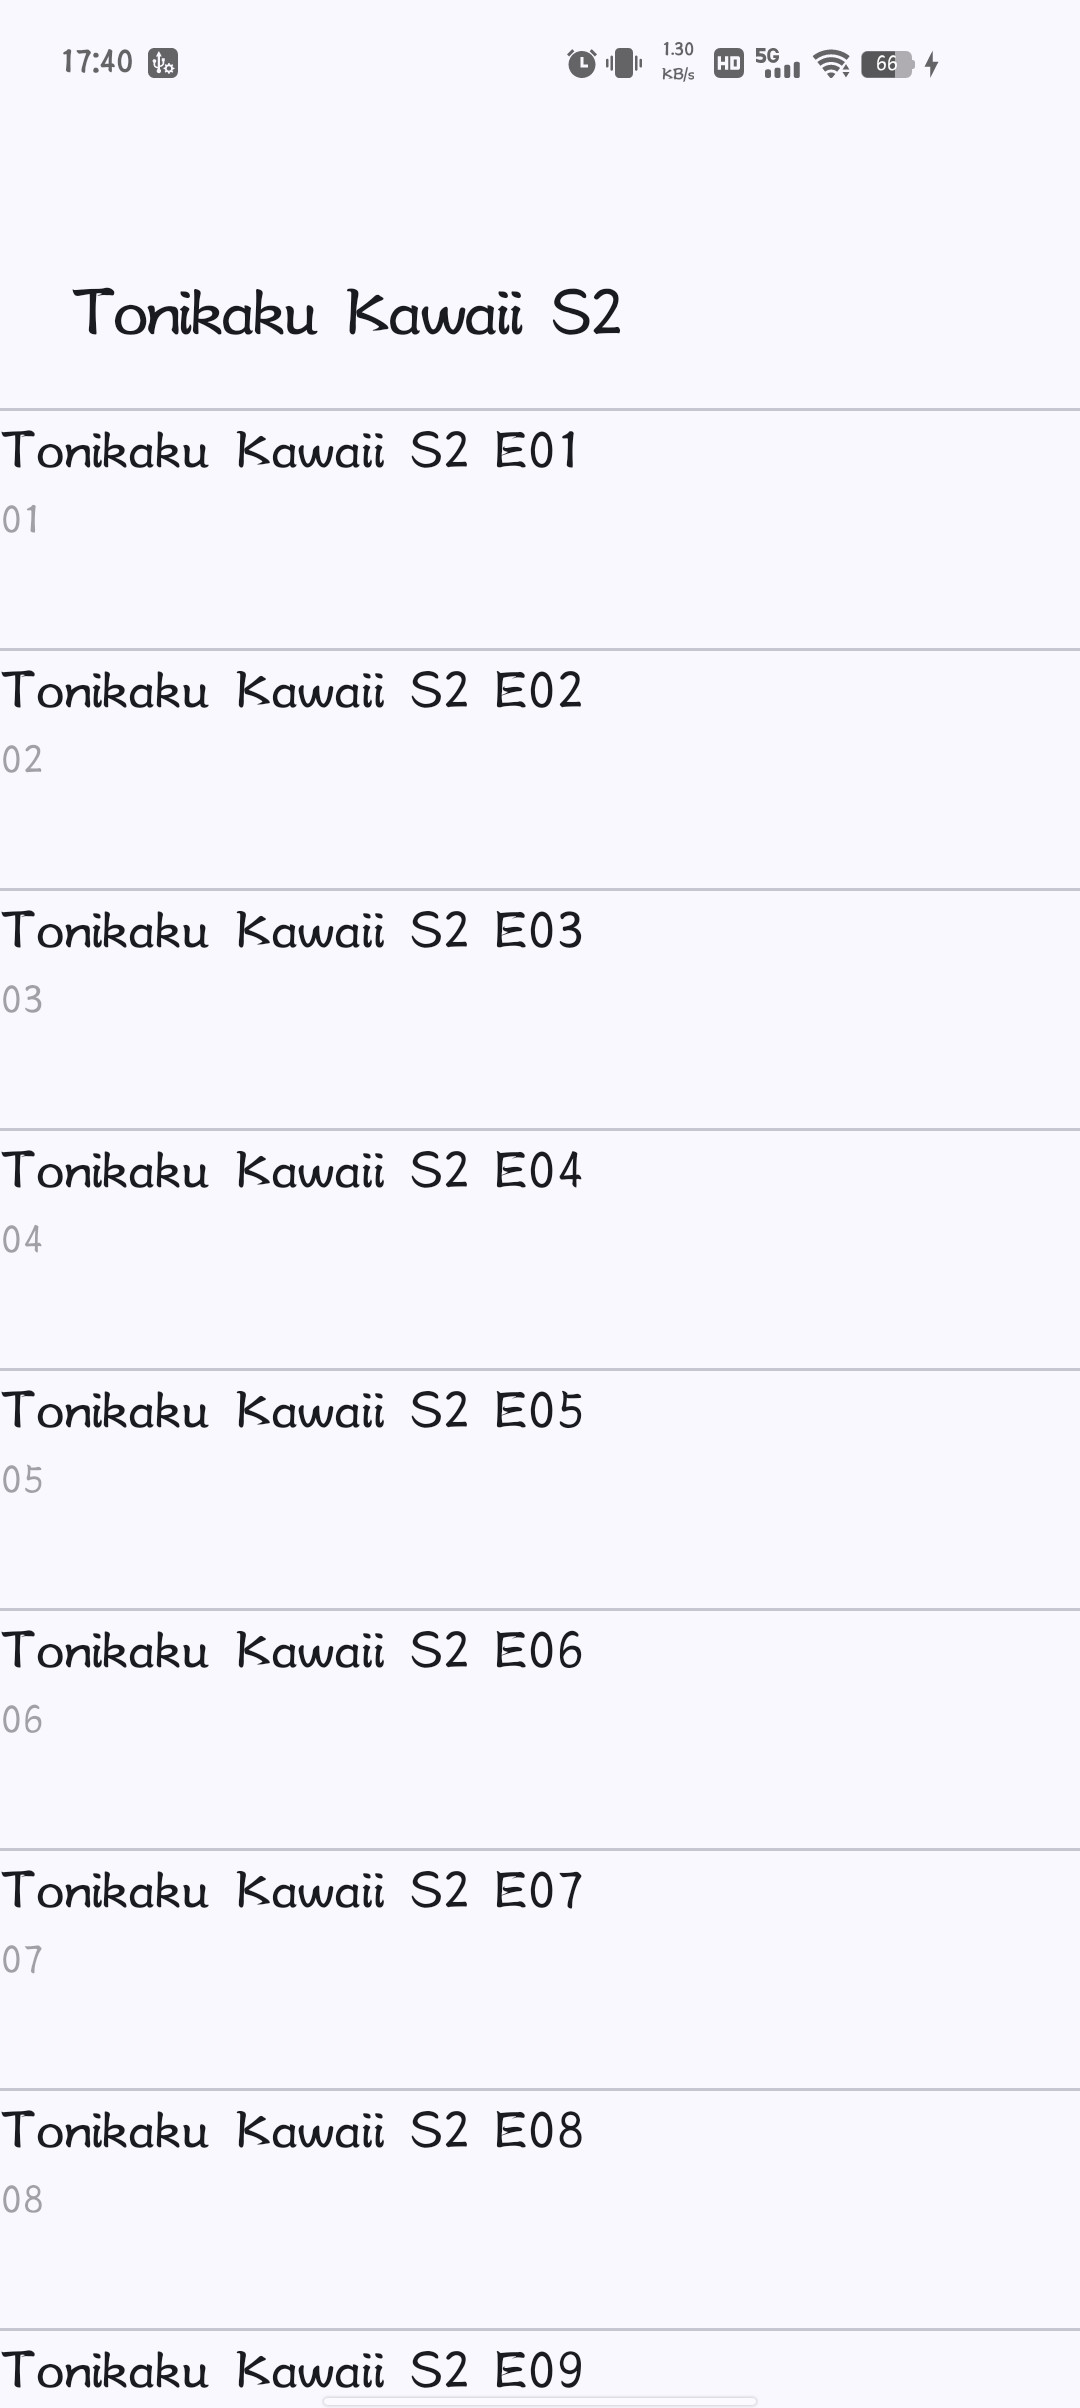
\includegraphics[width=0.4\linewidth]{assets/show-page.png}
    \caption{节目展示页面}
    \label{fig:show-page}
\end{figure}

节目展示页面也保持系统中一贯的页面设计风格,页面主要分成上下两个部分,缺少当前的播放状态。在页面上方的标题栏中,标题栏中展示了当前选择的节目标题。在页面中的列表中展示了当前选择节目中的视频列表,在列表中的每一项中展示了当前视频的标题和当前视频在该节目中的集数。在视频播放页面中没有设计同音乐播放中类似的播放状态栏是因为,视频的播放和音频的播放有着较大的不同,从逻辑上来说,视频播放很少有不需要看画面的时候,设计视频的后台播放意义不是很大,从实现上来说,后台播放视频和音乐在实现并没有任何的不同,不需要在视频的页面上重复的编写对应的代码。因此在这里我们会在进入视频播放页面时自动隐藏播放状态栏。

在节目展示页面中的点击任意视频就会进入到视频播放页面。视频播放页面如图所示。

\begin{figure}[htbp]
    \centering
    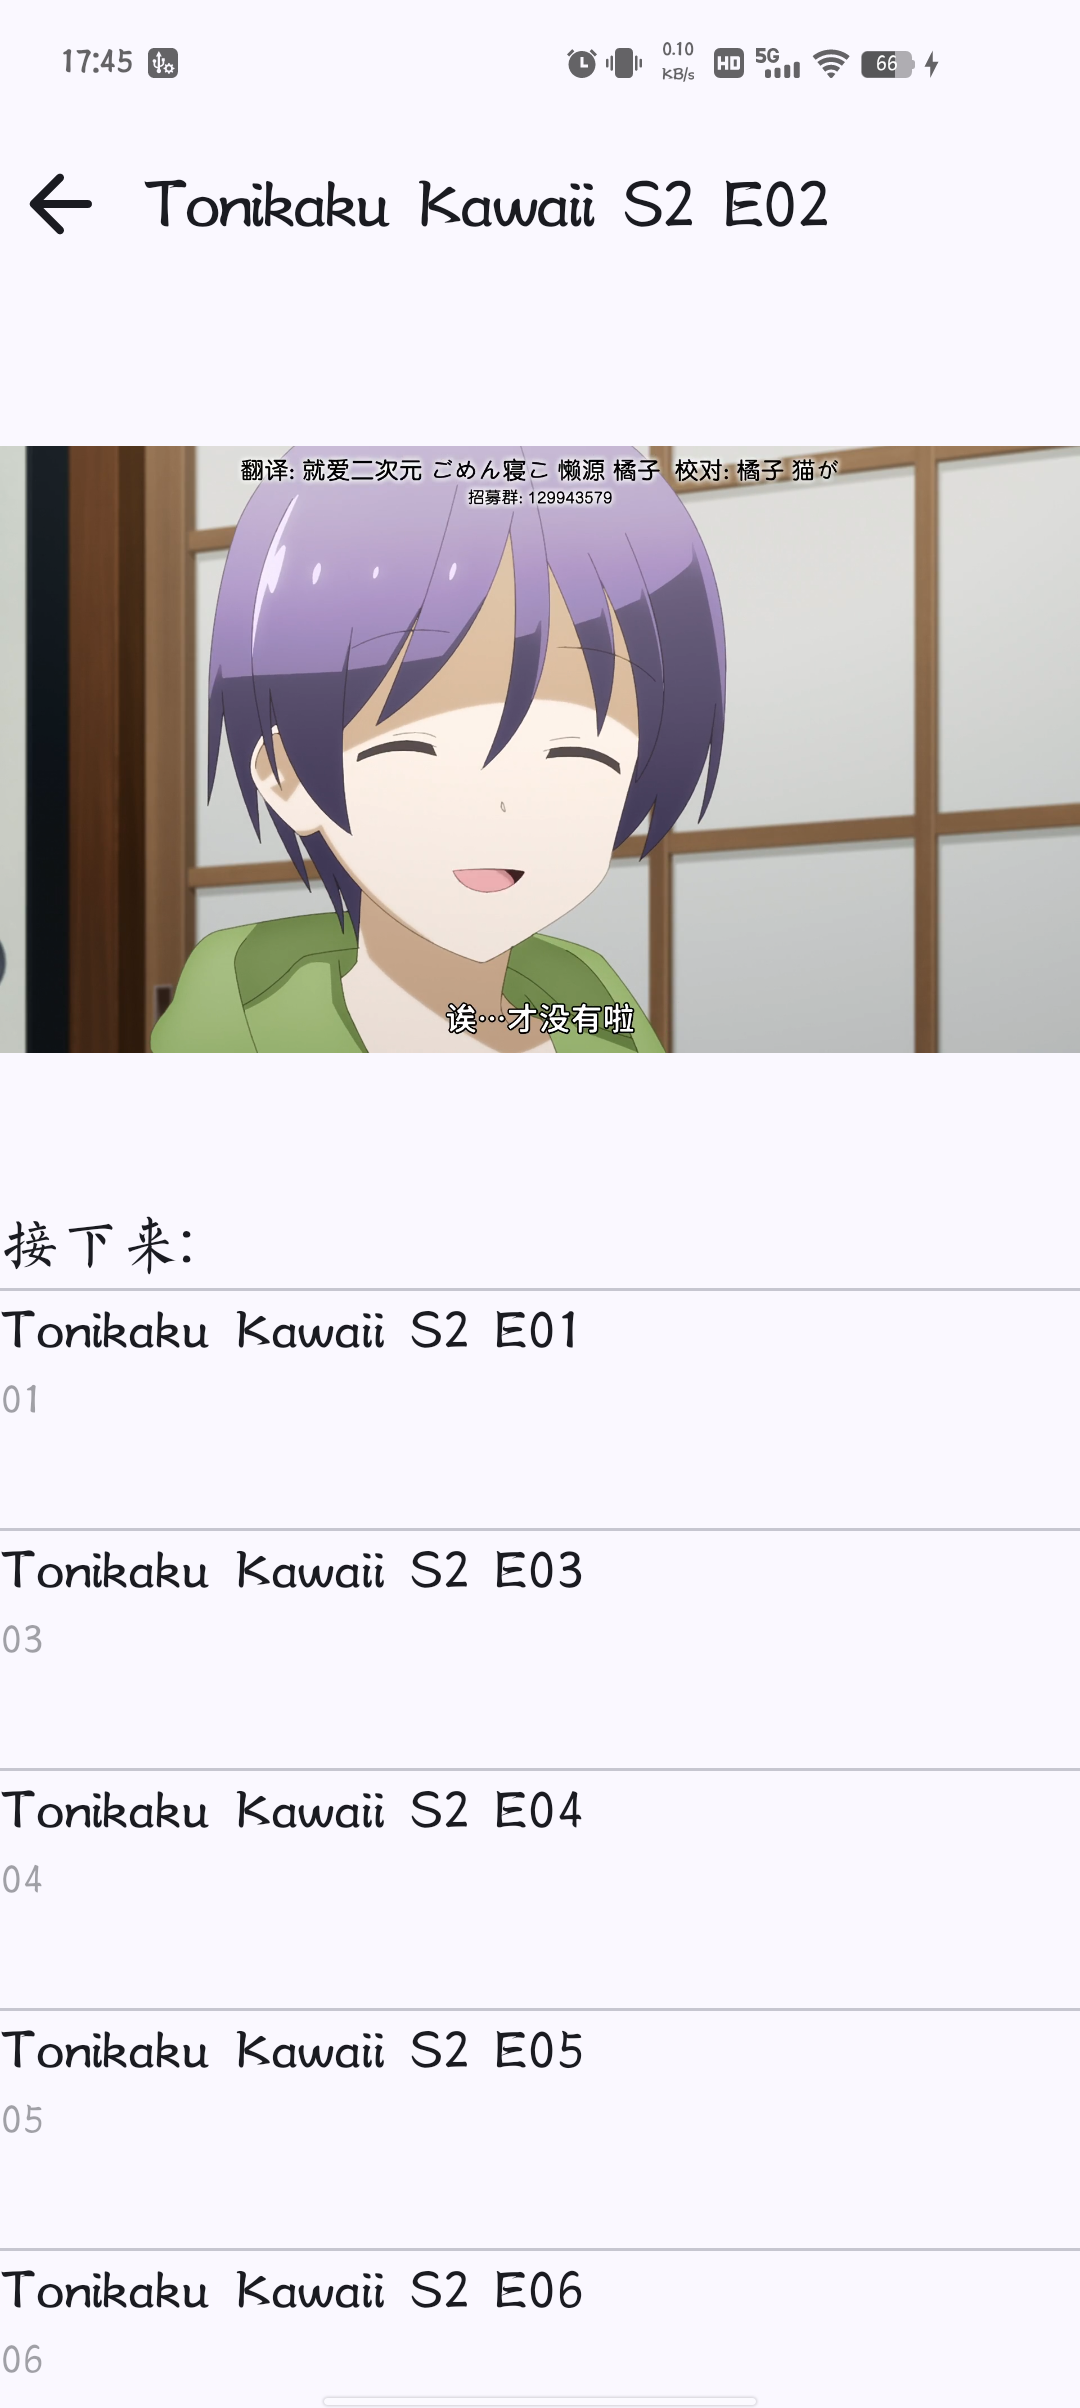
\includegraphics[width=0.4\linewidth]{assets/video-page.png}
    \caption{视频播放页面}
    \label{fig:video-page}
\end{figure}

视频播放页面在总体上也有三部分组成。最上面的仍然是标题栏,在标题栏中显示了当前播放视频的标题和一个返回上一页面的按钮。在页面的内容部分则分成两个部分,分别是视频的画面部分和接下来推荐观看的视频列表。接下来推荐观看的视频列表所展示的信息和节目页面所展示的信息是一致的,都是视频的标题和集数。

\end{document}